\documentclass{mjw}
\title{Enforced Invariant Confluence}
\author{Michael Whittaker}

\usepackage[hidelinks]{hyperref}
\usepackage[leqno]{amsmath}
\usepackage{../common/python}
\usepackage{amsfonts}
\usepackage{amssymb}
\usepackage{amsthm}
\usepackage{centernot}
\usepackage{environ}
\usepackage{etoolbox}
\usepackage{mathtools}
\usepackage{paralist}
\usepackage{stmaryrd}
\usepackage{subcaption}
\usepackage{tikz}

\usetikzlibrary{arrows}
\usetikzlibrary{backgrounds}
\usetikzlibrary{calc}
\usetikzlibrary{decorations.pathmorphing}
\usetikzlibrary{positioning}

\newtoggle{showtodos}
\toggletrue{showtodos}
\newcommand{\todo}[2][mwhittaker]{
  \iftoggle{showtodos}{\textcolor{red}{TODO(#1): #2}}{}
}
\NewEnviron{todoitemize}{
  \iftoggle{showtodos}{
    \begin{itemize}
      \BODY
    \end{itemize}
  }{}
}

\makeatletter
\newcommand{\leqnomode}{\tagsleft@true}
\newcommand{\reqnomode}{\tagsleft@false}
\makeatother

\newtheorem{theorem}{Theorem}
\newtheorem{claim}{Claim}
\renewcommand{\qedsymbol}{$\blacksquare$}

\newcommand{\clmref}[1]{Claim~\ref{clm:#1}}
\newcommand{\figref}[1]{Figure~\ref{fig:#1}}
\newcommand{\secref}[1]{Section~\ref{sec:#1}}
\newcommand{\appref}[1]{Appendix~\ref{app:#1}}
\newcommand{\thmref}[1]{Theorem~\ref{thm:#1}}

\newcommand{\defeq}{\stackrel{\mathclap{\normalfont\mbox{\scriptsize def}}}{=}}
\newcommand{\dom}[1]{\text{dom}}
\newcommand{\set}[1]{\left\{#1\right\}}
\newcommand{\setst}[2]{\left\{#1 \,\middle|\, #2\right\}}
\newcommand{\denote}[1]{\left\llbracket#1\right\rrbracket}
\newcommand{\benote}[1]{(\!|#1|\!)}
\newcommand{\etal}{\textit{et al}.}

\newcommand{\dbs}{\mathcal{D}}
\newcommand{\var}{\textsf{Var}}
\newcommand{\ints}{\mathbb{Z}}

\newcommand{\wimp}{W$\iinvariant$MP}
\newcommand{\imp}{$\iinvariant$MP}
\newcommand{\impaexp}{\textsf{Aexp}}
\newcommand{\impbexp}{\textsf{Bexp}}
\newcommand{\impcom}{\textsf{Com}}
\newcommand{\impskip}{\textsf{skip}}
\newcommand{\impif}[3]{\textsf{if}(#1)\set{#2}\textsf{else}\set{#3}}

\newcommand{\iinvariant}{\mathcal{I}}
\newcommand{\iconfluent}{$\iinvariant$-confluent}
\newcommand{\iconfluence}{$\iinvariant$-confluence}
\newcommand{\ipreservation}{$\iinvariant$-preservation}
\newcommand{\ipreserving}{$\iinvariant$-preserving}
\newcommand{\isafety}{$\iinvariant$-safety}
\newcommand{\isafe}{$\iinvariant$-safe}
\newcommand{\istrength}{$\iinvariant$-strength}
\newcommand{\istrong}{$\iinvariant$-strong}
\newcommand{\istrengthstar}{\istrength$^\ast$}
\newcommand{\istrongstar}{\istrong$^\ast$}
\newcommand{\iconvergence}{$\iinvariant$-convergence}
\newcommand{\iconvergent}{$\iinvariant$-convergent}

% Implication.
\tikzstyle{impl}=[-implies, double distance=3pt]

% Transaction.
\tikzstyle{txn}=[ultra thick, ->]

% Derived transaction.
\tikzstyle{dtxn}=[ultra thick, ->, dashed]

% Invariant node.
\newcommand{\inode}[3][]{
  \node[draw, shape=circle, minimum width=0.5cm, #1] (#2) at (#3) {};
  \node[fill, shape=circle, #1] () at (#3) {};
}

% Normal node.
\newcommand{\nnode}[3][]{
  \node[fill, shape=circle, #1] (#2) at (#3) {};
}



\tikzstyle{point}=[shape=circle, fill=blue, opacity=0.75]
\tikzstyle{vec}=[->, ultra thick, red, shorten >=0.1cm]

\begin{document}
\maketitle
\reqnomode

{\begin{abstract}
Strongly consistent systems are easy to reason about but face fundamental
limitations in availability and performance. Weakly consistent systems can be
implemented with very high performance but place a burden on the application
developer to reason about complex interleavings of execution.
\Invariantconfluence{} provides a formal framework for understanding when we
can get the best of both worlds. An \invariantconfluent{} object can be
efficiently replicated with no coordination needed to preserve its invariants.
However, actually determining whether or not an object is \invariantconfluent{}
is challenging: undecidable in general. In this paper, we establish conditions under
which a commonly used sufficient condition for \invariantconfluence{} is both
necessary and sufficient and use this condition to design (a) a general-purpose
interactive \invariantconfluence{} decision procedure and (b) a novel
sufficient condition that can be checked automatically. We then take a step
beyond \invariantconfluence{} and introduce a generalization of
\invariantconfluence{} called segmented \invariantconfluence{}, which allows us
to replicate non-\invariantconfluent{} objects with a small amount of
coordination. We implemented our theoretical findings in a prototype called
Lucy and found that our decision procedures efficiently handle common real-world workloads
including foreign key constraints, rollups, escrow transactions, and others.  We also
found that segmented \invariantconfluent{} replication can deliver up to an
order of magnitude more throughput than linearizable replication for low
contention workloads and comparable throughput for medium to high contention
workloads.
\end{abstract}
}
{\section{Research Vision}

At a very high level, this research tackles the same problems tackled by many
existing research projects like BOOM Analytics \cite{alvaro2010boom}, Bloom
\cite{alvaro2011consistency}, Bloom$^L$ \cite{conway2012logic}, TARDiS
\cite{crookstardis}, and IPA \cite{holt2016disciplined}:

\begin{quotation}
  \emph{How can we make writing weakly consistent programs more principled?}
\end{quotation}

BOOM Analytics, Bloom, and Bloom$^L$ use data-centric declarative programming
and program analysis based on the CALM theorem. TARDiS exposes the entire
history of divergent computations to users in a git-like system to empower them
to programmatically resolve conflicts. IPA uses a type system to ensure weakly
consistent data doesn't leak into strongly consistent data. \todo{Cite and
summarize \cite{balegas2015putting}, \cite{roy2015homeostasis},
\cite{li2012making}, and \cite{li2014automating}}

This system builds off existing research on CRDTs and \iconfluence{} to provide
a library of CRDTs, a language to express invariants over those CRDTs, the
ability to transactionally update the replicated CRDTs, and a decision
procedure to algorithmically determine whether the transactions are
\iconfluent{} with respect to the invariants, ensuring coordination free
execution if they are and potentially giving illustrative counterexamples when
they are not. A simple example of psuedocode written with this system may look
something like this:

\begin{Python}
# Create an increment/decrement counter CRDT.
x = PNCounter(0)

# Set the invariant that the counter must always be non-negative.
set_invariant(x >= 0)

# This transaction is invariant confluent and would be accepted by the system.
@transaction
def foo():
  x.increment(42)

# This transaction is not invariant confluent and would be rejected by the
# system.
@transaction
def bar():
  x.decrement(1)
\end{Python}

A more complex example of psuedocode may look something like this:

\begin{Python}
# A map from employee id to employee name.
employees = Map[Int, String]()
# The number of employees.
num_employees = PNCounter(0)
# Employee ids partitioned into teams.
teams = Set[Set[Int]]

# The number of employees has to equal the size of employees.
set_invariant(num_employees = employees.size())
# All ids in teams must appear in employees.
set_invariant(forall team in teams. team subset employees.keys())
# All teams must be disjoint.
set_invariant(forall a, b in teams. a != b => a intersect b = {})
# Every employee must be on a team
set_invariant(union(teams) = employees.keys())

# This transaction which adds a new employee would be checked for
# invariant-confluence by the system.
@transaction
def add_employee(name):
  id = employees.unique_id()
  employees.put(name, id)
  num_employees.increment(1)
  teams[0].add(id)
\end{Python}

This pseudocode brings up a lot of \emph{theoretical questions}...
\begin{inparaitem}
  \item What CRDTs and what operations can we support?
  \item What invariant languages can we support?
  \item Given the set of CRDTs and invariants, is determining invariant
    confluence even decidable?
  \item If so, can it be determined efficiently?
  \item If not, how can we limit the CRDTs, operations, or invariants to make
    it decidable?
\end{inparaitem}
...and a lot of \emph{systems questions}:
\begin{inparaitem}
  \item Is the system expressive enough to write real-world programs?
  \item Can the system be implemented as a library in an existing programming
    language?
  \item How do we architect and build an actual system out of this?
\end{inparaitem}

This research aims to answer these questions and develop a first-of-its-kind
system that allows programmers to write coordination free distributed systems
with more discipline than ever before.
}
{\section{Counters}
As a first step towards accomplishing our research vision, let's begin with a
\emph{simple} CRDT with \emph{simple} operations and a \emph{simple} invariant
language: PN-counters and linear equations and inequalities.

\subsection{Overview}
Recall that a \emph{G-Counter} CRDT is an increment-only counter
\cite{shapiro2011comprehensive}. A state-based G-Counter distributed across $n$
machines $1, 2, \ldots, n$ can be implemented as an $n$-tuple $(x_1, x_2,
\ldots, x_n)$ of natural numbers. The \emph{increment($k$) method} at machine
$i$ increments $x_i$ by $k$; the \emph{query method} returns the sum of the
tuple $\sum_{i=1}^n x_i$; and the \emph{merge method} computes the pairwise max
of two $n$-tuples.

A \emph{PN-Counter} CRDT is a counter which supports increments and decrements
and can be implemented as a pair $(p, n)$ of two G-Counters
\cite{shapiro2011comprehensive}. increment($x$) increments $p$ by $x$;
decrement($x$) increments $n$ by $x$; query returns $p - n$; and merge performs
a pairwise merge of $p$ and $n$.

Our \emph{invariant language} is formed from \emph{linear equations} (e.g. $x =
0$, $2x = y$, $-x + 42y - 2z = 16$) and \emph{inequalities} (e.g. $x > 0$, $2x
\leq y$, $-x + 42y - 2z \neq 16$) connected with the boolean connectives
\emph{and} ($\land$), \emph{or} ($\lor$), and \emph{not} ($\lnot$) (e.g.
$\lnot((\lnot(x < 0) \lor 2x = y) \land -x + 42y - 2z \geq 16)$).

A \emph{transaction} chooses a subset of variables and decrements or increments
each by a constant amount. For example, a transaction may increment $x$ by 1,
decrement $y$ by 42, and increment $z$ by 100.

Given a set of transactions and an invariant, we want to determine whether the
transactions are \iconfluent{} with respect to the invariant. For example, the
transaction that \emph{increments} $x$ by 1 is invariant confluent with respect
to the invariant $x > 0$, but the transaction that \emph{decrements} $x$ by 1
is not, as shown in \figref{decrement}.

\begin{figure}[h]
  \centering
  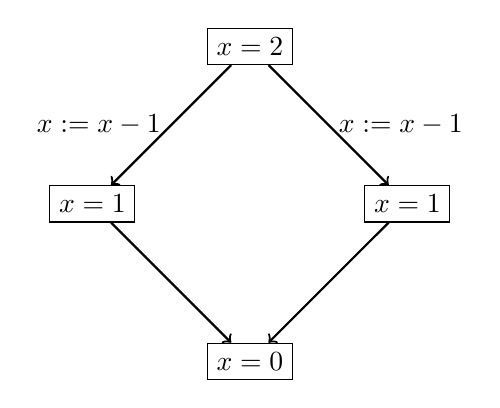
\begin{tikzpicture}
    % \draw (0, 0) grid (4, 4);
    \node[draw] (start)  at (2, 4) {$x=2$};
    \node[draw] (left)   at (0, 2) {$x=1$};
    \node[draw] (right)  at (4, 2) {$x=1$};
    \node[draw] (merged) at (2, 0) {$x=0$};

    \draw[thick, ->] (start) to node[left]  {$x := x - 1$} (left);
    \draw[thick, ->] (start) to node[right] {$x := x - 1$} (right);
    \draw[thick, ->] (left)  to (merged);
    \draw[thick, ->] (right) to (merged);
  \end{tikzpicture}
  \caption{
    A counterexample showing transaction $x := x - 1$ is not invariant
    confluent with respect to the invariant $x > 0$. The top, left, and right
    states satisfy the invariant, but the bottom state does not.
  }
  \label{fig:decrement}
\end{figure}

\subsection{Formalizing the Question}
\newcommand{\var}{\textsf{Var}}
\newcommand{\ints}{\mathbb{Z}}

Our invariant language is defined by the grammar in \figref{invariant-grammar}
which includes linear equations and inequalities over variables in a finite set
$\var$ and integer constants in $\ints$.

\begin{figure}[h]
  \centering

  \newcommand{\atom}{\textsf{atom}}
  \newcommand{\aexp}{\textsf{aexp}}
  \newcommand{\bexp}{\textsf{bexpr}}
  \begin{gather*}
    \begin{array}{rrll}
      \atom & ::= & k & \text{\emph{constants}} \\
            & |   & x & \text{\emph{variables}} \\
      &&& \\
      \aexp  & ::= & \atom         & \text{\emph{atom}} \\
             & |   & -\atom        & \text{\emph{negation}} \\
             & |   & \aexp + \aexp & \text{\emph{addition}} \\
             & |   & \aexp - \aexp & \text{\emph{subtraction}} \\
      &&& \\
      \bexp  & ::= & \aexp \leq \aexp  & \text{\emph{inequality}} \\
             & |   & \lnot \bexp       & \text{\emph{negation}} \\
             & |   & \bexp \land \bexp & \text{\emph{conjunction}} \\
             & |   & \bexp \lor \bexp  & \text{\emph{disjunction}} \\
    \end{array}
  \end{gather*}

  \caption{
    A grammar for our linear equation and linear inequality invariant language.
    Note that the comparison operators $=$, $\neq$, $<$, $>$, and $\geq$ are
    not included because they can be defined in terms of the existing
    operators.
  }
  \label{fig:invariant-grammar}
\end{figure}

A \emph{database state} is a total function $D: \var \to \ints$.  We say a
database state $D$ \emph{satisfies invariant} $I$ if $I$ evaluates to true
after all variables in $I$ have been replaced by their mapping in $D$.

A \emph{transaction} is a partial function $t: \var \rightharpoonup \ints$.
\emph{Applying a transaction} $t$ to database state $D$, denoted by $D \circ
t$, produces a new database state defined as follows:
\[
  (D \circ t)(x) \defeq \begin{cases*}
    D(x) + t(x) & $x \in \dom{}(t)$ \\
    D(x)        & otherwise
  \end{cases*}
\]
Note that transaction application is commutative. That is for all database
states $D$ and transactions $t_1$ and $t_2$, $D \circ t_1 \circ t_2 = D \circ
t_2 \circ t_1$.

A transaction chain $C$ created from a set of transactions $T$ is a sequence of
transactions $t_1, \ldots, t_n$ where $t_j \in T$ for $1 \leq j \leq n$. Let $D
\circ C$ be syntactic sugar for $D \circ t_1 \circ \cdots \circ t_n$. We say
$C$ \emph{satisfies invariant} $I$ starting at $D$ if for every prefix $C'$ of
$C$, $D \circ C'$ satisfies invariant $I$.

A set of transactions $T$ is \iconfluent{} with respect to invariant $I$ if for
all database states $D$ and chains $C_1$ and $C_2$ created from $T$, if $D$
satisfies $I$, $C_1$ satisfies $I$ starting at $D$, and $C_2$ satisfies $I$
starting at $D$, then so does $D \circ C_1 \circ C_2$.

\subsection{A Geometric Interpretation}
\newcommand{\inva}{x + y \geq 0}
\newcommand{\invb}{x - y \leq 0}
\newcommand{\invc}{x \geq 1}
\newcommand{\invd}{x \geq 3}
\newcommand{\inv}{(\inva \land \invb \land \invc) \lor (\invd)}

Sometimes, we can eyeball whether a transaction is \iconfluent{} with respect
to an invariant. Other times, not so much. For example, which transactions are
invariant confluent with respect to the invariant $\inv$? It's not immediately
clear.  Surprisingly, we can interpret the question ``Is $T$ \iconfluent{} with
respect to $I$?'' geometrically, and doing so will make answering the question
much easier!

Consider an invariant $I$ over $n$ variables $x_1, \ldots, x_n$. If we imagine
the values of the $n$ variables as an $n$-dimensional point, then we can draw
the set of points in $\ints^n$ that satisfy $I$. In fact, if we canonicalize
$I$ by eliminating negations and converting to conjunctive normal form, then
the set of points satisfying $I$ is the intersection (for $\land)$ and union
(for $\lor$) of the solutions to a set of linear equations and inequalities,
which is always straightforward to draw. For example, the set of points
satisfying $\inv$ is shown in \figref{geometric-example}.

\begin{figure}
  \newenvironment{griddedpic}{
    \begin{tikzpicture}
      \clip (-4, -1) rectangle (4, 4);
  }{
      \draw (-4, -1) grid (4, 4);
      \draw[ultra thick] (-4, 0) -- (4, 0);
      \draw[ultra thick] (0, -1) -- (0, 4);
    \end{tikzpicture}
  }

  \begin{subfigure}[c]{0.5\textwidth}
    \begin{griddedpic}
      \fill[red, opacity=0.4]
        (-10, 10) -- (10, -10) -- (10, 10) -- cycle;
    \end{griddedpic}
    \caption{$\inva$}
  \end{subfigure}
  \begin{subfigure}[c]{0.5\textwidth}
    \begin{griddedpic}
      \fill[blue, opacity=0.4]
        (-10, -10) -- (10, 10) -- (-10, 10) -- cycle;
    \end{griddedpic}
    \caption{$\invb$}
  \end{subfigure}

  \vspace{0.5cm}

  \begin{subfigure}[c]{0.5\textwidth}
    \begin{griddedpic}
      \fill[green, opacity=0.4]
        (-10, 1) -- (10, 1) -- (10, 10) -- (-10, 10) -- cycle;
    \end{griddedpic}
    \caption{$\invc$}
  \end{subfigure}
  \begin{subfigure}[c]{0.5\textwidth}
    \begin{griddedpic}
      \fill[orange, opacity=0.4]
        (-10, 3) -- (10, 3) -- (10, 10) -- (-10, 10) -- cycle;
    \end{griddedpic}
  \caption{$\invd$}
  \end{subfigure}

  \vspace{0.5cm}

  \begin{subfigure}[c]{\textwidth}
    \centering
    \begin{griddedpic}
      \fill[purple, opacity=0.4]
        (-1, 1) -- (-3, 3) -- (-10, 3) -- (-10, 10) -- (10, 10) -- (10, 3) --
        (3, 3) -- (1, 1) -- cycle;
    \end{griddedpic}
    \caption{$\inv$}
  \end{subfigure}

  \caption{An illustration of the solution to $\inv$.}
  \label{fig:geometric-example}
\end{figure}

Next, we can imagine a transaction $t$ as an $n$-dimensional vector $(k_{x_1},
\ldots, k_{x_n})$ where $t$ adds constant $k_{x_i}$ to variable $x_i$. Now, the
question of whether a set of transactions $T$ is \iconfluent{} with respect to
invariant $I$ has been reduced to the following question. Starting at an
arbitrary point $D$ in the solution space of $I$, if we can add vectors $t^1_1,
t^1_2, \ldots, t^1_m$ to $D$ and vectors $t^2_1, t^2_2, \ldots, t^2_n$ to $D$
all while staying in the solution space of $I$, then are we guaranteed that $D
+ t^1_1 + t^1_2 + \ldots + t^1_m + t^2_1 + t^2_2 + \ldots + t^2_n$ is in the
solution space of $I$?

Turning again to our example in \figref{geometric-example}, it is now clear
that any transaction $(k_x, k_y)$ where $y \geq 0$ and $|x| \leq y$ is
\iconfluent{} with respect to $\inv$. These are the vectors that point up and
not too far left or right.

\subsection{One is Enough}
Define a set of transactions $T$ to be $k$-\iconfluent{} with respect to
invariant $I$ if for all database states $D$ and chains $C_1$ and $C_2$ created
from $T$ of length at most $k$, if $D$ satisfies $I$, $C_1$ satisfies $I$
starting at $D$, and $C_2$ satisfies $I$ starting at $D$, then so does $D \circ
C_1 \circ C_2$.
%
A set of transactions $T$ is \iconfluent{} with respect to an invariant $I$ if
it is $k$-\iconfluent{} for all $k$. Thus, when reasoning about \iconfluent{}
transactions, we have to consider potentially large transaction chains which
can be a bit brain boggling. Reasoning about 1-\iconfluence{} is much easier
because we only have to consider a pair of transactions at a time. This
subsection proves a convenient lemma that 1-\iconfluence{} and \iconfluence{}
are equivalent.

\begin{theorem}
  For all sets of transactions $T$ and invariants $I$, T is 1-\iconfluent{} if
  and only if it is \iconfluent{}.
\end{theorem}
\begin{proof}
  The reverse direction is immediate from the definition of \iconfluence{}. For
  the forward direction, consider a set of transactions $T$ that is
  1-\iconfluent{} with respect to an invariant $I$, but assume for
  contradiction that $T$ is not \iconfluent{} with respect to $I$. That is,
  there exists a database state $D$ and two chains $C^1 = t^1_1, t^1_2, \ldots,
  t^1_m$ and $C^2 = t^2_1, t^2_2, \ldots, t^2_n$ such that $D$ satisfies $I$,
  $C^1$ satisfies $I$ starting at $D$, and $C^2$ satisfies $I$ starting at $D$
  but $D \circ C^1 \circ C^2$ does not.

  Let $C^z_j$ denote the prefix of $C^z$ of length $j$. We show by strong
  mathematical induction on $i$, that $D \circ C^1_j \circ C^2_k$ satisfies $I$
  for all $0 \leq j \leq m$, $0 \leq k \leq n$, and $0 \leq i = j + k \leq n +
  m$.
  %
  The base case, when $i = 0$, is trivial. $j = k = 0$, and $D \circ C^1_0
  \circ C^2_0 = D$ which satisfies $I$ by assumption.
  %
  For the inductive step, we wish to show for arbitrary $0 \leq j \leq m$, $0
  \leq k \leq n$, and $0 < i = j + k$ that $D \circ C^1_j \circ C^2_k$
  satisfies $I$. If $j = 0$, then $D \circ C^1_0 \circ C^2_k = D \circ C^2_k$
  satisfies $I$ by the assumption that $C^2$ satisfies $I$ starting at $D$, and
  likewise for when $k = 0$. Now consider $j, k > 0$. By the inductive
  hypothesis, we know
    (1) $D \circ C^1_{j-1} \circ C^2_{k-1}$,
    (2) $D \circ C^1_{j-1} \circ C^2_{k}$, and
    (3) $D \circ C^1_{j}   \circ C^2_{k-1}$
  all satisfy $I$. If we let (1) be our initial database state, $t^1_j$ be one
  chain, and $t^2_k$ be the other chain, then the 1-\iconfluence{} of $T$ tells
  us that $(1) \circ t^1_j \circ t^2_k = D \circ C^1_j \circ C^2_k$ satisfies
  $I$.
\end{proof}
}
{\section{\iconfluence{}, Formally}\label{sec:formalism}
Our invariant language is defined by the grammar in \figref{invariant-grammar}
which includes linear equations and inequalities over variables in a finite set
$\var$ and integer constants in $\ints$.

\begin{figure}[h]
  \centering

  \newcommand{\atom}{\textsf{atom}}
  \newcommand{\aexp}{\textsf{aexp}}
  \newcommand{\bexp}{\textsf{bexpr}}
  \begin{gather*}
    \begin{array}{rrll}
      \atom & ::= & k & \text{\emph{constants}} \\
            & |   & x & \text{\emph{variables}} \\
      &&& \\
      \aexp  & ::= & \atom         & \text{\emph{atom}} \\
             & |   & -\atom        & \text{\emph{negation}} \\
             & |   & \aexp + \aexp & \text{\emph{addition}} \\
             & |   & \aexp - \aexp & \text{\emph{subtraction}} \\
      &&& \\
      \bexp  & ::= & \aexp \leq \aexp  & \text{\emph{inequality}} \\
             & |   & \lnot \bexp       & \text{\emph{negation}} \\
             & |   & \bexp \land \bexp & \text{\emph{conjunction}} \\
             & |   & \bexp \lor \bexp  & \text{\emph{disjunction}} \\
    \end{array}
  \end{gather*}

  \caption{
    A grammar for our linear equation and linear inequality invariant language.
    Note that the comparison operators $=$, $\neq$, $<$, $>$, and $\geq$ are
    not included because they can be defined in terms of the existing
    operators.
  }
  \label{fig:invariant-grammar}
\end{figure}

A \emph{database state} is a total function $D: \var \to \ints$.  We say a
database state $D$ \emph{satisfies invariant} $I$, denoted $I(D)$, if $I$
evaluates to true after all variables in $I$ have been replaced by their
mapping in $D$. Let $\dbs$ denote the set of all database states.

A \emph{transaction} is a partial function $t: \var \rightharpoonup \ints$.
\emph{Applying a transaction} $t$ to database state $D$, denoted by $D \circ
t$, produces a new database state defined as follows:
\[
  (D \circ t)(x) \defeq \begin{cases*}
    D(x) + t(x) & $x \in \dom{}(t)$ \\
    D(x)        & otherwise
  \end{cases*}
\]
Note that transaction application is commutative. That is for all database
states $D$ and transactions $t_1$ and $t_2$, $D \circ t_1 \circ t_2 = D \circ
t_2 \circ t_1$.

A transaction chain $C$ created from a set of transactions $T$ is a sequence of
transactions $t_1, \ldots, t_n$ where $t_i \in T$ for $1 \leq i \leq n$. Let $D
\circ C$ be syntactic sugar for $D \circ t_1 \circ \cdots \circ t_n$. We say
$C$ \emph{satisfies invariant} $I$ starting at $D$, denoted $I(C @ D)$, if for
every prefix $C'$ of $C$, $D \circ C'$ satisfies invariant $I$.

A set of transactions $T$ is \iconfluent{} with respect to invariant $I$ if for
all database states $D$ and chains $C_1$ and $C_2$ created from $T$, if $D$
satisfies $I$, $C_1$ satisfies $I$ starting at $D$, and $C_2$ satisfies $I$
starting at $D$, then $D \circ C_1 \circ C_2$ satisfies $I$.
\todo{
  This isn't quite the definition of \iconfluence{} Bailis uses. Ponder whether
  this simpler definition is okay.
}

}
{\section{\iconfluence{}, Geometrically}\label{sec:geometry}
\newcommand{\inva}{x + y \geq 0}
\newcommand{\invb}{x - y \leq 0}
\newcommand{\invc}{y \geq 1}
\newcommand{\invd}{y \geq 3}
\newcommand{\inv}{(\inva \land \invb \land \invc) \lor (\invd)}

Sometimes---like with the two examples from the previous section---we can
eyeball whether a transaction is \iconfluent{} with respect to an invariant.
Other times, not so much. For example, which transactions are \iconfluent{}
with respect to the invariant $\inv$? It's not immediately clear.
Surprisingly, we can interpret the question ``Is $T$ \iconfluent{} with respect
to $I$?'' geometrically, and doing so will make answering the question much
easier!

Consider databases over $n$ variables $\var = \set{x_1, \ldots, x_n}$. We can
imagine a database $D$ as the $n$-dimensional point $(D(x_i), \ldots, D(x_n))$.
For example, if $\var = \set{x, y}$, then the database $\set{x:1, y:2}$
corresponds to the two-dimensional point $(1, 2)$.

We can imagine $I$ as the set of points (or databases) in $\ints^n$ that
satisfy $I$. For example, the invariant $x + y = 2$ corresponds to the set of
two-dimensional points $(k_x, k_y)$ where $k_x + k_y = 2$. This corresponds to
the set of databases $\set{x:k_x, y:k_y}$ where $k_x + k_y = 2$.

Moreover, if we canonicalize $I$ by eliminating negations and converting to
conjunctive normal form, then the set of points satisfying $I$ is the
intersection (for $\land)$ and union (for $\lor$) of the solutions to a set of
linear equations and inequalities, which is always straightforward to draw. For
example, the set of points satisfying $\inv$ is shown in
\figref{geometric-example}.

\begin{figure}
  \newenvironment{griddedpic}{
    \begin{tikzpicture}[scale=0.4]
      \clip (-4, -1) rectangle (4, 4);
  }{
      \draw (-4, -1) grid (4, 4);
      \draw[ultra thick] (-4, 0) -- (4, 0);
      \draw[ultra thick] (0, -1) -- (0, 4);
    \end{tikzpicture}
  }

  \begin{subfigure}[b]{0.24\textwidth}
    \centering
    \begin{griddedpic}
      \fill[red, opacity=0.4]
        (-10, 10) -- (10, -10) -- (10, 10) -- cycle;
    \end{griddedpic}
    \caption{$\inva$}
  \end{subfigure}
  \begin{subfigure}[b]{0.24\textwidth}
    \centering
    \begin{griddedpic}
      \fill[blue, opacity=0.4]
        (-10, -10) -- (10, 10) -- (-10, 10) -- cycle;
    \end{griddedpic}
    \caption{$\invb$}
  \end{subfigure}
  \begin{subfigure}[b]{0.24\textwidth}
    \centering
    \begin{griddedpic}
      \fill[green, opacity=0.4]
        (-10, 1) -- (10, 1) -- (10, 10) -- (-10, 10) -- cycle;
    \end{griddedpic}
    \caption{$\invc$}
  \end{subfigure}
  \begin{subfigure}[b]{0.24\textwidth}
    \centering
    \begin{griddedpic}
      \fill[orange, opacity=0.4]
        (-10, 3) -- (10, 3) -- (10, 10) -- (-10, 10) -- cycle;
    \end{griddedpic}
  \caption{$\invd$}

  \end{subfigure}
  \begin{subfigure}[b]{\textwidth}
    \centering
    \begin{griddedpic}
      \fill[purple, opacity=0.4]
        (-1, 1) -- (-3, 3) -- (-10, 3) -- (-10, 10) -- (10, 10) -- (10, 3) --
        (3, 3) -- (1, 1) -- cycle;
    \end{griddedpic}
    \caption{$\inv$}
  \end{subfigure}

  \caption{An illustration of the solution to $\inv$.}
  \label{fig:geometric-example}
\end{figure}

Next, we can imagine a transaction $t = \set{x_1:k_{x_1}, \ldots, x_n:k_{x_n}}$
as an $n$-dimensional vector $(k_{x_1}, \ldots, k_{x_n})$. For example, given
the invariant $x + y = 2$, the transaction $\set{x:2, y:4}$ corresponds to the
vector $(2, 4)$. Applying a transaction $t$ to a database $D$ can be understood
as adding the vector representing $t$ to the point representing $D$.  For
example, applying the transaction $\set{x:2, y:4}$ to the database $\set{x:10,
y:20}$ corresponds to adding the vector $(2, 4)$ to the point $(10, 20)$
bringing us to the point $(12, 24)$.

Now, the question of whether a set of transactions $T$ is \iconfluent{} with
respect to invariant $I$ has been reduced to the following question. Starting
at an arbitrary point $D$ in the solution space of $I$, if we can add vectors
$t_1, t_2, \ldots, t_m$ to $D$ and vectors $u_1, u_2, \ldots, u_n$ to $D$ all
while staying in the solution space of $I$, then are we guaranteed that $D +
t_1 + t_2 + \ldots + t_m + u_1 + u_2 + \ldots + u_n$ is in the solution space
of $I$?

Turning again to our example in \figref{geometric-example}, it is now clear
that any transaction $\set{x:k_x, y:k_y}$ where $y \geq 0$ and $|x| \leq y$ is
\iconfluent{} with respect to $\inv$. These correspond to the vectors $(k_x,
k_y)$ that point up and not too far left or right.
}
{\section{One is Enough}\label{sec:oneisenough}
Define a set of transactions $T$ to be $k$-\iconfluent{} with respect to
invariant $I$ if for all database states $D$ and chains $C_1$ and $C_2$ created
from $T$ of length at most $k$, if $D$ satisfies $I$, $C_1$ satisfies $I$
starting at $D$, and $C_2$ satisfies $I$ starting at $D$, then $D \circ
C_1 \circ C_2$ satisfies $I$.
%
A set of transactions $T$ is \iconfluent{} with respect to an invariant $I$ if
it is $k$-\iconfluent{} for all $k$. Thus, when reasoning about \iconfluent{}
transactions, we have to consider potentially large transaction chains which
can be a bit brain boggling. Reasoning about 1-\iconfluence{} is much easier
because we only have to consider a pair of transactions at a time. This
subsection proves a convenient lemma that 1-\iconfluence{} and \iconfluence{}
are equivalent.

\begin{theorem}\label{thm:one-is-enough}
  For all sets of transactions $T$ and invariants $I$, T is 1-\iconfluent{}
  with respect to $I$ if and only if it is \iconfluent{} with respect to $I$.
\end{theorem}
\begin{proof}
  The reverse direction is immediate from the definition of \iconfluence{}. For
  the forward direction, consider a set of transactions $T$ that is
  1-\iconfluent{} with respect to an invariant $I$. Consider an arbitrary
  database state $D$ and two chains $C^t = t_1, t_2, \ldots, t_m$ and $C^u =
  u_1, u_2, \ldots, u_n$ such that $D$ satisfies $I$, $C^t$ satisfies $I$
  starting at $D$, and $C^u$ satisfies $I$ starting at $D$. We show $D \circ
  C^t \circ C^u$ satisfies $I$.

  Let $C^z_j$ denote the prefix of $C^z$ of length $j$. We show by strong
  mathematical induction on $i$, that $D \circ C^t_j \circ C^u_k$ satisfies $I$
  for all $0 \leq j \leq m$, $0 \leq k \leq n$, and $0 \leq i = j + k \leq n +
  m$.
  %
  The base case, when $i = 0$, is trivial. $j = k = 0$, and $D \circ C^t_0
  \circ C^u_0 = D$ which satisfies $I$ by assumption.
  %
  For the inductive step, we wish to show for arbitrary $0 \leq j \leq m$, $0
  \leq k \leq n$, and $i = j + k$ that $D \circ C^t_j \circ C^u_k$ satisfies
  $I$. If $j = 0$, then $D \circ C^t_0 \circ C^u_k = D \circ C^u_k$ satisfies
  $I$ by the assumption that $C^u$ satisfies $I$ starting at $D$, and likewise
  for when $k = 0$. Now consider $j, k > 0$. By the inductive hypothesis, we
  know
    (1) $D \circ C^t_{j-1} \circ C^u_{k-1}$,
    (2) $D \circ C^t_{j-1} \circ C^u_{k}$, and
    (3) $D \circ C^t_{j}   \circ C^u_{k-1}$
  all satisfy $I$. If we let (1) be our initial database state, $t_j$ be one
  chain, and $u_k$ be the other chain, then the 1-\iconfluence{} of $T$ tells
  us that $(1) \circ t_j \circ u_k = D \circ C^t_j \circ C^u_k$ satisfies
  $I$.
\end{proof}

\newcommand{\baseedges}{
  \begin{scope}[on background layer]
    \draw[txn] (03) -- (13) node[midway, above]{$u_1$};
    \draw[txn] (13) -- (23) node[midway, above]{$u_2$};
    \draw[txn] (23) -- (33) node[midway, above]{$u_3$};
    \draw[txn] (03) -- (02) node[midway, left]{$t_1$};
    \draw[txn] (02) -- (01) node[midway, left]{$t_2$};
    \draw[txn] (01) -- (00) node[midway, left]{$t_3$};
    \draw[dtxn] (00) -- (30);
    \draw[dtxn] (33) -- (30);
  \end{scope}
}

\begin{figure}[h]
  \centering
  \newcommand{\onescale}{1.1}

  \begin{subfigure}[b]{0.49\textwidth}
    \centering
    \begin{tikzpicture}[scale=\onescale]
      \foreach \x/\y in {
             1/3, 2/3, 3/3,
        0/2,
        0/1,
        0/0%
      } {
        \inode{\x\y}{\x, \y}
      }
      \foreach \x/\y in {0/3} {
        \inode[red]{\x\y}{\x, \y}
      }
      \nnode{30}{3, 0}
      \baseedges{}
    \end{tikzpicture}
    \caption{$i = 0$}
    \label{fig:one-is-enough-base}
  \end{subfigure}
  \begin{subfigure}[b]{0.49\textwidth}
    \centering
    \begin{tikzpicture}[scale=\onescale]
      \foreach \x/\y in {
        0/3,      2/3, 3/3,
        %
        0/1,
        0/0%
      } {
        \inode{\x\y}{\x, \y}
      }
      \foreach \x/\y in {0/2, 1/3} {
        \inode[red]{\x\y}{\x, \y}
      }
      \nnode{30}{3, 0}
      \baseedges{}
    \end{tikzpicture}
    \caption{$i=1$}
    \label{}
  \end{subfigure}

  \begin{subfigure}[b]{0.3\textwidth}
    \centering
    \begin{tikzpicture}[scale=\onescale]
      \foreach \x/\y in {
        0/3, 1/3,      3/3,
        0/2,
        %
        0/0%
      } {
        \inode{\x\y}{\x, \y}
      }
      \foreach \x/\y in {0/1, 1/2, 2/3} {
        \inode[red]{\x\y}{\x, \y}
      }
      \nnode{30}{3, 0}
      \baseedges{}
      \draw[txn] (02) -- (12) node[midway, above] {$u_1$};
      \draw[txn] (13) -- (12) node[midway, left]  {$t_1$};
    \end{tikzpicture}
    \caption{$i=2$}
    \label{}
  \end{subfigure}
  \begin{subfigure}[b]{0.3\textwidth}
    \centering
    \begin{tikzpicture}[scale=\onescale]
      \foreach \x/\y in {
        0/3, 1/3, 2/3,
        0/2, 1/2,
        0/1%
        %
      } {
        \inode{\x\y}{\x, \y}
      }
      \foreach \x/\y in {0/0, 1/1, 2/2, 3/3} {
        \inode[red]{\x\y}{\x, \y}
      }
      \nnode{30}{3, 0}
      \baseedges{}
      \draw[txn] (02) -- (12) node[midway, above] {$u_1$};
      \draw[txn] (13) -- (12) node[midway, left]  {$t_1$};
      \draw[txn] (01) -- (11) node[midway, above] {$u_1$};
      \draw[txn] (12) -- (11) node[midway, left]  {$t_2$};
      \draw[txn] (12) -- (22) node[midway, above] {$u_2$};
      \draw[txn] (23) -- (22) node[midway, left]  {$t_1$};
    \end{tikzpicture}
    \caption{$i=3$}
    \label{}
  \end{subfigure}
  \begin{subfigure}[b]{0.3\textwidth}
    \centering
    \begin{tikzpicture}[scale=\onescale]
      \foreach \x/\y in {
        0/3, 1/3, 2/3, 3/3,
        0/2, 1/2, 2/2,
        0/1, 1/1,
        0/0%
      } {
        \inode{\x\y}{\x, \y}
      }
      \foreach \x/\y in {1/0, 2/1, 3/2} {
        \inode[red]{\x\y}{\x, \y}
      }
      \nnode{30}{3, 0}
      \baseedges{}
      \draw[txn] (02) -- (12) node[midway, above] {$u_1$};
      \draw[txn] (13) -- (12) node[midway, left]  {$t_1$};
      \draw[txn] (01) -- (11) node[midway, above] {$u_1$};
      \draw[txn] (12) -- (11) node[midway, left]  {$t_2$};
      \draw[txn] (12) -- (22) node[midway, above] {$u_2$};
      \draw[txn] (23) -- (22) node[midway, left]  {$t_1$};
      \draw[txn] (00) -- (10) node[midway, above] {$u_1$};
      \draw[txn] (11) -- (10) node[midway, left]  {$t_3$};
      \draw[txn] (11) -- (21) node[midway, above] {$u_2$};
      \draw[txn] (22) -- (21) node[midway, left]  {$t_2$};
      \draw[txn] (22) -- (32) node[midway, above] {$u_3$};
      \draw[txn] (33) -- (32) node[midway, left]  {$t_1$};
    \end{tikzpicture}
    \caption{$i=4$}
    \label{}
  \end{subfigure}

  \begin{subfigure}[b]{0.49\textwidth}
    \centering
    \begin{tikzpicture}[scale=\onescale]
      \foreach \x/\y in {
        0/3, 1/3, 2/3, 3/3,
        0/2, 1/2, 2/2, 3/2,
        0/1, 1/1, 2/1,
        0/0, 1/0%
      } {
        \inode{\x\y}{\x, \y}
      }
      \foreach \x/\y in {2/0, 3/1} {
        \inode[red]{\x\y}{\x, \y}
      }
      \nnode{30}{3, 0}
      \baseedges{}
      \draw[txn] (02) -- (12) node[midway, above] {$u_1$};
      \draw[txn] (13) -- (12) node[midway, left]  {$t_1$};
      \draw[txn] (01) -- (11) node[midway, above] {$u_1$};
      \draw[txn] (12) -- (11) node[midway, left]  {$t_2$};
      \draw[txn] (12) -- (22) node[midway, above] {$u_2$};
      \draw[txn] (23) -- (22) node[midway, left]  {$t_1$};
      \draw[txn] (00) -- (10) node[midway, above] {$u_1$};
      \draw[txn] (11) -- (10) node[midway, left]  {$t_3$};
      \draw[txn] (11) -- (21) node[midway, above] {$u_2$};
      \draw[txn] (22) -- (21) node[midway, left]  {$t_2$};
      \draw[txn] (22) -- (32) node[midway, above] {$u_3$};
      \draw[txn] (33) -- (32) node[midway, left]  {$t_1$};
      \draw[txn] (10) -- (20) node[midway, above] {$u_2$};
      \draw[txn] (21) -- (20) node[midway, left]  {$t_3$};
      \draw[txn] (21) -- (31) node[midway, above] {$u_3$};
      \draw[txn] (32) -- (31) node[midway, left]  {$t_2$};
    \end{tikzpicture}
    \caption{$i=5$}
    \label{}
  \end{subfigure}
  \begin{subfigure}[b]{0.49\textwidth}
    \centering
    \begin{tikzpicture}[scale=\onescale]
      \foreach \x/\y in {
        0/3, 1/3, 2/3, 3/3,
        0/2, 1/2, 2/2, 3/2,
        0/1, 1/1, 2/1, 3/1,
        0/0, 1/0, 2/0%
      } {
        \inode{\x\y}{\x, \y}
      }
      \inode[red]{30}{3, 0}
      \baseedges{}
      \draw[txn] (02) -- (12) node[midway, above] {$u_1$};
      \draw[txn] (13) -- (12) node[midway, left]  {$t_1$};
      \draw[txn] (01) -- (11) node[midway, above] {$u_1$};
      \draw[txn] (12) -- (11) node[midway, left]  {$t_2$};
      \draw[txn] (12) -- (22) node[midway, above] {$u_2$};
      \draw[txn] (23) -- (22) node[midway, left]  {$t_1$};
      \draw[txn] (00) -- (10) node[midway, above] {$u_1$};
      \draw[txn] (11) -- (10) node[midway, left]  {$t_3$};
      \draw[txn] (11) -- (21) node[midway, above] {$u_2$};
      \draw[txn] (22) -- (21) node[midway, left]  {$t_2$};
      \draw[txn] (22) -- (32) node[midway, above] {$u_3$};
      \draw[txn] (33) -- (32) node[midway, left]  {$t_1$};
      \draw[txn] (10) -- (20) node[midway, above] {$u_2$};
      \draw[txn] (21) -- (20) node[midway, left]  {$t_3$};
      \draw[txn] (21) -- (31) node[midway, above] {$u_3$};
      \draw[txn] (32) -- (31) node[midway, left]  {$t_2$};
      \draw[txn] (20) -- (30) node[midway, above] {$u_3$};
      \draw[txn] (31) -- (30) node[midway, left]  {$t_3$};
    \end{tikzpicture}
    \caption{$i=6$}
    \label{}
  \end{subfigure}

  \caption{Illustration of the proof of \thmref{one-is-enough}.}
  \label{fig:one-is-enough}
\end{figure}

\figref{one-is-enough} visualizes the proof of \thmref{one-is-enough} using
\emph{state diagrams}. In a state diagram, each dot represents a database state
$D$, and we draw an edge labelled $t$ from database $D$ to database $D'$ if $D
\circ t = D'$. We circle a database dot if we know it satisfies the invariant
and leave it uncircled otherwise.

\figref{one-is-enough} illustrates an initial database $D$ (top-left dot), a
chain $C^t = \set{t_1, t_2, t_3}$ (the left edge), a chain $C^u = \set{u_1,
u_2, u_3}$ (the top edge), and $D \circ C^t \circ C^u$ (the bottom-right dot).
By assumption, we know $D$, $D \circ C^t_1$, $D \circ C^t_2$, $D \circ C^t$, $D
\circ C^u_1$, $D \circ C^u_2$, and $D \circ C^u$ satisfy the invariant, and we
want to show that $D \circ C^t \circ C^u$ satisfies the invariant.
\figref{one-is-enough-base} illustrates the base case of
\thmref{one-is-enough}; each of the other six state diagrams illustrate one
inductive step of \figref{one-is-enough}. In each inductive step, we exploit
the fact that $T$ is 1-\iconfluent{} to conclude that some set of intermediate
databases satisfy the invariant.
}
{\section{A Solution}\label{sec:solution}
This paper posed the question: how do we write an algorithm to decide whether a
set of PN-Counter increment/decrement transactions are \iconfluent{} with
respect to an invariant expressed as a formula of linear equations and
inequalities?  Now that we're armed with an intuitive (\secref{counters}) and
formal (\secref{formalism}) understanding of the problem, a geometric
interpretation (\secref{geometry}), and a useful lemma (\secref{oneisenough}),
we're in a perfect position to present a solution!

In a nutshell, our algorithm translates a set of transactions $T$ and invariant
$I$ into a universally quantified invariant $F$ in prenex normal form where $F$
is a tautology if and only if $T$ is 1-\iconfluent{} with respect to $I$. Thus,
by \thmref{one-is-enough}, $F$ is a tautology if and only if $T$ is
\iconfluent{} with respect to $I$. Our algorithm then uses Z3 \cite{de2008z3}
to check if $F$ is a tautology.

The algorithm for constructing $F$ is best explained by way of example.
Consider a simple case where $I = x + y \geq 0$, and $T$ consists of a single
transaction $t$ which increments $x$ by 1 and $y$ by 2. Our algorithm
constructs the following formula
\begin{align}
  & \forall x.\> \forall y.\>                \label{eq:vars} \\
  & \forall dx_1.\> \forall dy_1.\>          \label{eq:dvars1} \\
  & \forall dx_2.\> \forall dy_2.\>          \label{eq:dvars2} \\
  & (dx_1 = 1 \land dy_1 = 2) \land {}       \label{eq:t1} \\
  & (dx_2 = 1 \land dy_2 = 2) \implies {}    \label{eq:t2} \\
  & x + y \geq 0 \implies {}                 \label{eq:i} \\
  & x + dx_1 + y + dy_1 \geq 0 \implies {}   \label{eq:i1} \\
  & x + dx_2 + y + dy_2 \geq 0 \implies {}   \label{eq:i2} \\
  & x + dx_1 + dx_2 + y + dy_1 + dy_2 \geq 0 \label{eq:i12}
\end{align}
where
\begin{itemize}
  \item
    \eqref{eq:vars} universally quantifies the free variables in $I$.

  \item
    \eqref{eq:dvars1} and \eqref{eq:dvars2} universally quantify variables
    $dx_1$ and $dx_2$ for each free variable $x$ in the invariant $I$.
    Intuitively, if the invariant has free variables $a, \ldots, z$, then the
    variables $da_1, \ldots, dz_1$ represent the increments and decrements of
    one transaction and $da_2, \ldots, dz_2$ represent the increments and
    decrements of another transaction.

  \item
    \eqref{eq:t1} and \eqref{eq:t2} assert that $dx_1$, $dy_1$, $dx_2$, and
    $dy_2$ must take on values consistent with $t$. Specifically, $x$ must be
    incremented by 1, and $y$ must be incremented by $2$.

  \item
    \eqref{eq:i} is $I$. Intuitively, it predicates our implication on the
    assumption that the current database state satisfies the invariant.

  \item
    \eqref{eq:i1} is $I$ with every variable $\alpha$ replaced with $\alpha +
    d\alpha_1$.  Intuitively, it predicates our implication on the assumption
    that if we apply the first transaction, our database still satisfies the
    invariant.  \eqref{eq:i2} is symmetric to \eqref{eq:i1} but for the second
    transaction instead of the first.

  \item
    \eqref{eq:i12} is $I$ with every variable $\alpha$ replaced with $\alpha +
    d\alpha_1 + d\alpha_2$. Intuitively, it says that if we apply both the
    transactions, we continue to satisfy our invariant.
\end{itemize}

To summarize, the formula encodes the statement that for all database state
$(x, y)$ for all transactions $t_1 = (dx_1, dy_1) \in T$, and for all
transactions $t_2 = (dx_2, dy_2) \in T$, if $(x, y)$, $(x + dx_1, y + dy_1)$,
and $(x + dx_2, y + dy_2)$ satisfy the invariant, then so does $(x + dx_1 +
dx_2, y + dy_1 + dy_2)$. In other words, the formula is nothing more than a
restatement of the definition of 1-\iconfluence!

}
{\section{\imp{}}\label{sec:imp}
So far, we've modelled a transaction $t: \var \rightharpoonup \ints$ as a
partial function from variables to integers. Intuitively, a transaction chooses
some \emph{fixed} subset of variables and increments and decrements each by
some \emph{fixed} amount. We'll call these kinds of transactions \emph{fixed
transactions}. While simple, fixed transactions are \emph{inexpressive}. We can
model, for example, a transaction that increments $x$ by 42 and decrements $y$
by 14, but we \emph{can't} model a transaction that increments $y$ by $x$ or a
transaction that increments $y$ by 1 whenever $x$ is positive and increments
$z$ whenever $x$ is negative.

In this subsection, we introduce a simple imperative programming language
\imp{}\footnote{That's IMP \cite{winskel1993formal} with an $\iinvariant{}$.}.
Instead of looking at fixed transactions, we'll look at \imp{}
transactions---transactions written in \imp{}---and ask ourselves the question
of how do determine whether a set of \imp{} transactions is \iconfluent{} with
respect to some invariant.

\begin{figure}[h]
  \centering
  \begin{gather*}
    \begin{array}{rrll}
      \impaexp\;
        a & ::= & k       & \text{\emph{constant}} \\
          & |   & x       & \text{\emph{variable}} \\
          & |   & read(x) & \text{\emph{database read}} \\
          & |   & a + a   & \text{\emph{addition}} \\
          & |   & a - a   & \text{\emph{subtraction}} \\
          & |   & - a     & \text{\emph{negation}} \\
      &&& \\
      \impbexp\;
        b & ::= & \textsf{true}  & \text{\emph{true}} \\
          & |   & \textsf{false} & \text{\emph{false}} \\
          & |   & a \odot a      & \text{\emph{linear constraint}} \\
          & |   & \lnot b        & \text{\emph{negation}} \\
          & |   & b \lor b       & \text{\emph{disjunction}} \\
          & |   & b \land b      & \text{\emph{conjunction}} \\
      &&& \\
      \impcom\;
        c  & ::= & \impskip        & \text{\emph{skip}} \\
           & |   & x := a          & \text{\emph{assignment}} \\
           & |   & add(x, a)       & \text{\emph{database adds}} \\
           & |   & c; c            & \text{\emph{sequence}} \\
           & |   & \impif{b}{c}{c} & \text{\emph{conditional}} \\
      &&& \\
      \odot & ::= & =    \vert
                    \neq \vert
                    <    \vert
                    \leq \vert
                    >    \vert
                    \geq & \text{\emph{comparator}}
    \end{array}
  \end{gather*}

  \caption{
    A grammar for \imp{}: a simple imperative transaction language inspired by
    IMP \cite{winskel1993formal} and $\mathcal{L}$ \cite{roy2015homeostasis}.
    The language consists of arithmetic expressions $\impaexp{}$, boolean
    expressions $\impbexp{}$, and commands $\impcom{}$.
  }
  \label{fig:imp-grammar}
\end{figure}

The syntax of \imp{} is defined by the grammar in \figref{imp-grammar}. The
semantics of \imp{} can be defined denotationally. That is, we can define a
denotational semantics $\denote{\cdot}$ where for an \imp{} program $c$,
$\denote{c}: (\var \to \ints) \to (\var \rightharpoonup \ints)$ is a function
from a database to a fixed transaction. Defining these semantics is left as an
exercise to the reader.  See \cite{cs6110sp2016lecture19} for guidance.
\todo{Define, explicitly, the denotational semantics if need be.}

\emph{Applying an \imp{} transaction} $c$ to database state $D$, denoted by $D
\circ c$, is defined as $D \circ c \defeq D \circ (\denote{c}(D))$.  Note that
unlike fixed transaction application, \imp{} transaction application is
\emph{not} commutative! For example, consider the database $D=\set{(x, 0)}$ and
\imp{} transactions $c_1 = add(x, 1)$ and $c_2 = add(x, read(x))$.
\[
  D \circ c_1 \circ c_2
    = \set{(x, 1)} \circ c_2
    = \set{(x, 2)}
    \neq \set{(x, 1)}
    = \set{(x, 0)} \circ c_1
    = D \circ c_2 \circ c_1
\]

An \imp{} transaction chain $B$ created from a set of \imp{} transactions $T$
is a sequence of \imp{} transactions $c_1, \ldots, c_n$ where $c_i \in T$ for
$1 \leq i \leq n$. Each \imp{} transaction chain $B$ starting with database
state $D$ has a corresponding fixed transaction chain $C$ denoted
$\denote{B}(D)$. Let $D_i = D \circ c_1 \circ \cdots \circ c_i$. Then, the
corresponding fixed transaction chain is $\denote{c_1}(D_0), \ldots,
\denote{c_n}(D_{n-1})$. We say $B$ \emph{satisfies invariant} $I$ starting at
$D$, denoted $I(B@D)$, if the corresponding fixed transaction chain $C$
satisfies invariant $I$ starting at $D$.

We say a set of \imp{} transactions $T$ is \iconfluent{} with respect to
invariant $I$ if for all database states $D$, all \imp{} chains $B_1$ and $B_2$
created from $T$, and corresponding fixed transaction chains $C_1$ and $C_2$,
if $D$ satisfies $I$, $B_1$ satisfies $I$ starting at $D$, and $B_2$ satisfies
$I$ starting at $D$, then $D \circ C_1 \circ C_2$ satisfies $I$. We define
$k$-\iconfluence{} similar to how we did in \secref{counter-one}.

Now that we've formalized what it means for a set of \imp{} transactions to be
\iconfluent{} with respect to some invariant, how do we determine
\iconfluence{} algorithmically? One initial hunch would be to apply the same
technique from \secref{solution} with slight modification. Unfortunately,
\clmref{imp-1-iconfluence} presents a challenge.

\begin{claim}\label{clm:imp-1-iconfluence}
  For \imp{} transactions, $1$-\iconfluence $\centernot \implies$ \iconfluence.
\end{claim}
\begin{proof}
  Consider the following invariant and \imp{} transactions:
  \begin{align*}
    I &\defeq
      (-2 \leq x \leq 2 \land y = 0) \lor (x = 1 \land 0 \leq y \leq 2) \\
    c_1 &\defeq \impif{x = 0 \land y = 0}{
      add(x, 1)
    }{\impif{x = 1 \land y = 0} {
      add(y, 1)
    }{
      \impskip
    }} \\
    c_2 &\defeq \impif{x = 0 \land y = 0}{
      add(x, -1)
    }{\impif{x = 1 \land y = 0} {
      add(y, 1)
    }{
      \impskip
    }}
  \end{align*}

  $T = \set{c_1, c_2}$ is $1$-\iconfluent{} with respect to $I$, but not
  $2$-\iconfluent{} with respect to $I$. Proving this is easiest if we
  interpret \imp{} transactions geometrically, as we did with fixed
  transactions.

  As before, invariants over $n$ variables correspond to a set of points in
  $\ints^n$; for example, $I$ is visualized in \figref{iviz}. An \imp{}
  transaction $c$ can be thought of as vector valued functions $c: \ints^n \to
  \ints^n$ that maps each point in $\ints^n$ to a $n$-dimensional vector. For
  example, $c_1$ and $c_2$ are visualized in \figref{c1viz} and \figref{c2viz}.
  The visualization of $c_1$ has two vectors. The $(1, 0)$ vector originating
  at the origin corresponds to $c_1$ adding $1$ to $x$ whenever $x = 0 \land y
  = 0$. Similarly, the $(0, 1)$ originating at $(1, 0)$ corresponds to $c_1$
  adding $1$ to $y$ whenever $x = 1 \land y = 0$.

  Using this geometric interpretation, it's easy to perform a brute-force check
  that $T$ is $1$-\iconfluent with respect to $I$. However, consider the
  transaction chains $B_1 = \set{c_1, c_2}$ and $B_2 = \set{c_2, c_1}$ starting
  in database state $D = (0, 0)$. We know that
  \begin{itemize}
    \item $D = (0, 0)$ satisfies $I$,
    \item $D \circ c_1 = (0, 1)$ satisfies $I$,
    \item $D \circ c_1 \circ c_2 = (1, 1)$ satisfies $I$,
    \item $D \circ c_2 = (-1, 0)$ satisfies $I$, and
    \item $D \circ c_2 \circ c_1 = (-1, 0)$ satisfies $I$,
  \end{itemize}
  but $D \circ C_1 \circ C_2 = D \circ (1, 0) \circ (0, 1) \circ (-1, 0) \circ
  (0, 0) = (0, 1)$ does not satisfy $I$. Therefore, $T$ is not 2-\iconfluent
  with respect to $I$ and is therefore not \iconfluent with respect to $I$.
\end{proof}

\todo{
  \clmref{imp-1-iconfluence} puts us in a bit of pickle. Think about how to get
  out of it. Maybe we check for $k$-\iconfluence for some $k$ and then use a
  reservation system to bound the amount of divergence between replicas? That
  doesn't seem to make sense for a system with high transaction throughput.
  Maybe there are some other tricks we can play?
}

\begin{figure}[h]
  \centering

  \newcommand{\gridandpoints}{
    \draw[ultra thick] (-2, 0) -- (2, 0);
    \draw[ultra thick] (0, 0) -- (0, 2);
    \draw (-2, 0) grid (2, 2);
    \foreach \x/\y in {-2/0, -1/0, 0/0, 1/0, 2/0, 1/1, 1/2} {
      \node[point] (\x-\y) at (\x, \y) {};
    }
  }

  \begin{subfigure}[c]{0.3\textwidth}
    \centering
    \begin{tikzpicture}
      \gridandpoints{}
    \end{tikzpicture}
    \caption{Visualization of $I$.}
    \label{fig:iviz}
  \end{subfigure}
  \begin{subfigure}[c]{0.3\textwidth}
    \centering
    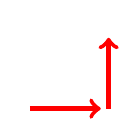
\begin{tikzpicture}
      \gridandpoints{}
      \draw[vec] (0, 0) -- (1, 0);
      \draw[vec] (1, 0) -- (1, 1);
    \end{tikzpicture}
    \caption{Visualization of $c_1$.}
    \label{fig:c1viz}
  \end{subfigure}
  \begin{subfigure}[c]{0.3\textwidth}
    \centering
    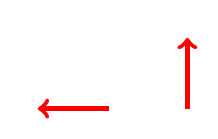
\begin{tikzpicture}
      \gridandpoints{}
      \draw[vec] (0, 0) -- (-1, 0);
      \draw[vec] (1, 0) -- (1, 1);
    \end{tikzpicture}
    \caption{Visualization of $c_2$.}
    \label{fig:c2viz}
  \end{subfigure}

  \caption{
    A geometric interpretation of $I$, $c_1$, and $c_2$ from
    \clmref{imp-1-iconfluence}. $I$ corresponds to a subset of $\ints^2$. $c_1$
    and $c_2$ correspond to vector valued functions of type $\ints^2 \to
    \ints^2$.
  }
  \label{fig:icviz}
\end{figure}

}
{\section{\wimp{}}\label{sec:wimp}
We began this paper by looking at fixed transactions and concluded in
\thmref{one-is-enough} that if a set of fixed transactions is 1-\iconfluent{}
with respect to an invariant $I$, then it is also \iconfluent{}. Then in
\secref{imp}, we enriched transactions from simple fixed partial functions
to full-blown programs written in \imp{}. Unfortunately, this increase in
expressiveness came at the cost of the nice fact that 1-\iconfluence{} is
equivalent to \iconfluence{}, as we saw in \thmref{imp-1-iconfluence}.

Perhaps \imp{} is too powerful of a transaction language. In particular, it has
two powerful features that fixed transactions do not have. First, \imp{} has
conditionals allowing the control flow of an \imp{} program to depend on the
database against which it is run. Second, even without conditionals, the
behavior of an \imp{} transaction can still depend on the database state
against which it is run. For example, the behavior of the transaction $add(x,
read(x))$ depends on the initial value of $x$, even though the transaction does
not use a conditional.

Perhaps if we strip \imp{} of some its features, we'll regain the equivalence
of 1-\iconfluence{} and \iconfluence{}. That is, perhaps there is an
intermediate language more powerful than fixed transactions but weaker than
\imp{} for which 1-\iconfluence{} is equivalent to \iconfluence{}.

In this subsection, we'll consider one such language, \wimp{}: a weakened
version of \imp{}. Then, we'll conclude that for \wimp{}---as for
\imp{}---1-\iconfluence{} does not imply \iconfluence{}.

Formally, \wimp{} is \imp{} without variables, boolean expressions, skip,
assignment, and conditionals. Moreover, each database variable can be added to
at most once. Essentially, \wimp{} programs get to add a single arithmetic
expression to each database variable. While weaker than \imp{} programs,
\wimp{} programs are more powerful than fixed transactions because arithmetic
expressions can include database reads and therefore \wimp{} programs can
depend on the initial state of the database. In fact, if we remove database
reads from \wimp{}, we get a language of fixed transactions.

Since \wimp{} is a subset of \imp{}, all the definitions from \imp{} carry over
directly for \wimp{}. Also note that like \imp{}, \wimp{} transaction
application is not commutative.

As mentioned above, \wimp{} is not weak enough to enjoy the equivalence of
1-\iconfluence{} and \iconfluence{}: a fact we now prove.

\begin{theorem}\label{thm:wimp-1-iconfluence}
  For \wimp{} transactions, $1$-\iconfluence $\centernot \implies$ \iconfluence.
\end{theorem}
\begin{proof}
  Consider the following invariant and \wimp{} transactions:
  \begin{align*}
    I   &\defeq x \neq 0 \lor y = 0 \\
    c_1 &\defeq y.add(1) \\
    c_2 &\defeq x.add(read(x) + 1) \\
    c_3 &\defeq x.add(read(x) - 1)
  \end{align*}

  As usual, we can visualize invariants and transactions geometrically, as
  shown in \figref{wimp-icviz}. We can perform a brute-force case analysis over
  all pairs of transactions and all points to show $T = \set{c_1, c_2, c_3}$ is
  1-\iconfluent{} with respect to $I$. This is left as exercise to the reader.

  However, consider the \wimp{} chains $B_1 = \set{c_2, c_1}$ and $B_2 =
  \set{c_3, c_1}$ in database $D = (0, 0)$. We know that
  \begin{itemize}
    \item $D = (0, 0)$ satisfies $I$,
    \item $D \circ c_2 = (1, 0)$ satisfies $I$,
    \item $D \circ c_2 \circ c_1 = (1, 1)$ satisfies $I$,
    \item $D \circ c_3 = (-1, 0)$ satisfies $I$, and
    \item $D \circ c_3 \circ c_1 = (-1, 1)$ satisfies $I$,
  \end{itemize}
  but $D \circ C_1 \circ C_2 = D \circ (1, 0) \circ (0, 1) \circ (-1, 0) \circ
  (0, 1) = (0, 2)$ does not satisfy $I$. Therefore, $T$ is not 2-\iconfluent
  with respect to $I$ and is therefore not \iconfluent with respect to $I$.
\end{proof}

\todo{
  We're in a pickle again! I think this result also might suggest that the
  claims in \cite{balegas2015putting} are wrong? More likely, I'm
  misunderstanding the paper.
}

\newcommand{\width}{2}
\newcommand{\smallwidth}{1}
\newcommand{\height}{2}

\newcommand{\gridxy}{
  \draw[ultra thick] (-\width, 0) -- (\width, 0);
  \draw[ultra thick] (0, -\height) -- (0, \height);
  \draw (-\width, -\height) grid (\width, \height);
}

\newcommand{\forxy}[1]{
  \foreach \x in {-\width, ..., -1} {
    \foreach \y in {-\height, ..., \height} { #1 } }
  \foreach \x in {1, ..., \width} {
    \foreach \y in {-\height, ..., \height} { #1 } }
  \foreach \x in {0} {
    \foreach \y in {0} { #1 } }
}

\newcommand{\forxysmall}[1]{
  \foreach \x in {-\smallwidth, ..., -1} {
    \foreach \y in {-\height, ..., \height} { #1 } }
  \foreach \x in {1, ..., \smallwidth} {
    \foreach \y in {-\height, ..., \height} { #1 } }
  \foreach \x in {0} {
    \foreach \y in {0} { #1 } }
}

\begin{figure}[h]
  \centering
  \newcommand{\thescale}{0.7}

  \begin{subfigure}[b]{0.24\textwidth}
    \centering
    \begin{tikzpicture}[scale=\thescale]
      \gridxy{}
      \forxy{\node[point] (\x-\y) at (\x, \y) {};}
    \end{tikzpicture}
    \caption{Visualization of $I$.}
    \label{fig:wimp-iviz}
  \end{subfigure}
  \begin{subfigure}[b]{0.24\textwidth}
    \centering
    \begin{tikzpicture}[scale=\thescale]
      \gridxy{}
      \forxy{\node[point] (\x-\y) at (\x, \y) {};}
      \forxy{\draw[vec] (\x, \y) -- (\x, \y + 1);}
    \end{tikzpicture}
    \caption{Visualization of $c_1$.}
    \label{fig:wimp-c1viz}
  \end{subfigure}
  \begin{subfigure}[b]{0.24\textwidth}
    \centering
    \begin{tikzpicture}[scale=\thescale]
      \gridxy{}
      \forxy{\node[point] (\x-\y) at (\x, \y) {};}
      \forxysmall{\draw[vec] (\x, \y) -- (\x + \x + 1, \y);}
    \end{tikzpicture}
    \caption{Visualization of $c_2$.}
    \label{fig:wimp-c2viz}
  \end{subfigure}
  \begin{subfigure}[b]{0.24\textwidth}
    \centering
    \begin{tikzpicture}[scale=\thescale]
      \gridxy{}
      \forxy{\node[point] (\x-\y) at (\x, \y) {};}
      \forxysmall{\draw[vec] (\x, \y) -- (\x + \x - 1, \y);}
    \end{tikzpicture}
    \caption{Visualization of $c_3$.}
    \label{fig:wimp-c3viz}
  \end{subfigure}

  \caption{
    A geometric interpretation of $I$, $c_1$, $c_2$, and $c_3$ from
    \thmref{wimp-1-iconfluence}. Note that the visualizations include only a
    subset of the points satisfying $I$ and that not all vectors are drawn.
  }
  \label{fig:wimp-icviz}
\end{figure}

}
{\section{\iconfluence{} Alternatives}
\begin{todoitemize}
  \item \todo{\istrength $\implies$ \istrengthstar?}
  \item \todo{\iconfluence $\implies$ 1-\iconvergence?}
  \item \todo{Find something between \isafety{} and \iconfluence.}
  \item \todo{1-iconfluence with derived txns to start}
\end{todoitemize}

\begin{itemize}
  \item \textbf{0-\isafety.}
    $\forall D, D', c.\>
      I(D) \land
      I(D') \implies
      I(D \circ \denote{c}(D'))$

  \item \textbf{k-\isafety.}
    $\forall D, D', B, C, c.\>
       C = \denote{B}(D) \land
       |B| \geq k \land
       I(B @ D') \implies
       I(C @ D) \land
       I(D \circ C \circ \denote{c}{D' \circ C})$

  \item \textbf{\isafety.}
    $\forall D, D', B, C, c.\>
       C = \denote{B}(D) \land
       I(B @ D') \implies
       I(D \circ C \circ \denote{c}(D' \circ C))$

  \item \textbf{\ipreservation.} $\forall D, c.\>
       I(D) \implies
       I(D \circ \denote{c}(D))$

  \item \textbf{\iconfluence.}
    $\forall D, B_1, B_2, C_1, C_2. \>
       C_1 = \denote{B_1}(D) \land
       C_2 = \denote{B_2}(D) \land
       I(B_1 @ D) \land
       I(B_2 @ D) \implies
       I(D \circ C_1 \circ C_2)$

  \item \textbf{k-\iconfluence.}
    $\forall D, B_1, B_2, C_1, C_2. \>
       C_1 = \denote{B_1}(D) \land
       C_2 = \denote{B_2}(D) \land
       |B_1|, |B_2| \leq k \land
       I(B_1 @ D) \land
       I(B_2 @ D) \implies
       I(D \circ C_1 \circ C_2)$

  \item \textbf{1-\iconfluence.}
    $\forall D, c_1, c_2.\>
       I(D) \land
       I(D \circ \denote{c_1}(D)) \land
       I(D \circ \denote{c_2}(D)) \implies
       I(D \circ \denote{c_1}(D) \circ \denote{c_2}(D))$

  \item \textbf{\istrengthstar{} \cite{gotsman2016cause}.}
    \leqnomode
    \begin{flalign*}
      & \exists G_0 \subseteq \dbs \times \dbs.& \\
      & G_0(I) \subseteq I \land{} & \tag*{S2.} \\
      & \forall c, D, D'.\>
          D \in I \land
          (D, D') \in G_0^* \implies
          (D', D' \circ \denote{c}(D)) \in G_0 & \tag*{S3.}
    \end{flalign*}
    \reqnomode
    where $I$ is viewed as a set of database states.

  \item \textbf{\istrength{} \cite{gotsman2016cause}.}
    \leqnomode
    \begin{flalign*}
      & \exists G_0 \subseteq \dbs \times \dbs. & \\
      & G_0(I) \subseteq I \land{} & \tag*{T2.} \\
      & \forall c.\>
        \exists P_1, \ldots, P_n \subseteq \dbs.\>
        \exists Q_1, \ldots, Q_n \subseteq \dbs.\> & \tag*{T3.} \\
      & \quad I \subseteq \cup_{i=1}^n P_i \land {} & \tag*{T3b.} \\
      & \quad \forall i \in \set{1, \ldots, n}.\> & \\
      & \quad \quad P_i \subseteq Q_i \land {} & \tag*{T3c.} \\
      & \quad \quad G_0(Q_i) \subseteq Q_i \land {} & \tag*{T3d.} \\
      & \quad \quad Q_i \times \denote{c}(P_i)(Q_i) \subseteq G_0 & \tag*{T3e.}
    \end{flalign*}
    \reqnomode
    where $I$ is viewed as a set of database states.

  \item \textbf{1-\iconvergence.}
    $\forall D, D', D'', c', c''.\>
      I(D) \land I(D') \land I(D'') \land
      I(D \circ \denote{c'}(D')) \land
      I(D \circ \denote{c''}(D'')) \implies
      I(D \circ \denote{c'}(D') \circ \denote{c''}(D''))$
\end{itemize}

\begin{claim}\label{clm:0-isafety-implies-istrengthstar}
  0-\isafety $\implies$ \istrengthstar.
\end{claim}
\begin{proof}
  Consider an arbitrary set of \imp{} transactions $T$ that is 0-\isafe{} with
  respect to invariant $I$. We show $T$ is \istrongstar{} with respect to $I$.
  Let $G_0 = I \times I$. S2 holds trivially: $G_0(I) = I
  \subseteq I$. Consider an arbitrary $c$, $D$, and $D'$ where $D \in I$ and
  $(D, D') \in G_0^*$.
  \begin{align*}
    & D \in I \land (D, D') \in G_0^*  \\
    &\implies D \in I \land D' \in I \tag{Definition of $G_0$} \\
    &\implies D' \in I \land D' \circ \denote{c}(D) \in I \tag{0-\isafety} \\
    &\implies (D', D' \circ \denote{c}(D)) \in G_0 \tag{Definition of $G_0$}
  \end{align*}
\end{proof}

\begin{claim}\label{clm:istrengthstar-not-implies-0-isafety}
  \istrengthstar $\centernot\implies$ 0-\isafety
\end{claim}
\begin{proof}
  Consider a database over a single variable $x$. For convenience, we'll denote
  database states as integers. Let
  \begin{itemize}
    \item
      $G \defeq \set{(0, 0), (0, 2)} \cup \setst{(a, b)}{a \geq 2, b \geq a}$
    \item
      $I \defeq x = 0 \lor x \geq 2$, and
    \item
      the single \imp{} transaction $c \defeq
      \impif{read(x)=0}{add(x, 0)}{add(x, 1)}$.
  \end{itemize}

  First note that $c$ is \istrengthstar{} with respect to $I$. S2 holds
  trivially. To show S3 holds, consider an arbitrary pair $a, b \in G_0^*$.
  \begin{itemize}
    \item \textbf{Case $a = 0, b = 0$.}
      $0 \circ \denote{c}(0) = 0 + 0 = 0$ and $(0, 0) \in G_0$.
    \item \textbf{Case $a = 0, b >= 2$.}
      $b \circ \denote{c}(0) = b + 0 = b$ and $(b, b) \in G_0$.
    \item \textbf{Case $a \geq 2, b >= a$.}
      $b \circ \denote{c}(a) = b + a$ and $(b, b + a) \in G_0$.
  \end{itemize}

  Now note that $c$ is not 0-\isafe{} with respect to $I$. Notably, $I(0)$ and
  $I(2)$, but $0 \circ \denote{c}(2) = 0 + 1 = 1$ and $\lnot I(1)$.
\end{proof}

\begin{claim}\label{clm:istrengthstar-implies-ipreservation}
  \istrengthstar $\implies$ \ipreservation
\end{claim}
\begin{proof}
  Consider a set of transactions $T$ that is \istrongstar{} with respect to
  invariant $I$ with relation $G_0$. Consider an arbitrary database $D$ that
  satisfies $I$ and an arbitrary \imp{} transaction $c$. $(D, D) \in G_0^*$,
  so by S3, $(D, D \circ \denote{c}(D)) \in G_0$. By S2, $I(D \circ \denote{c}(D))$.
\end{proof}

\begin{claim}\label{clm:istrengthstar-implies-iconfluence}
  \istrengthstar{} $\implies$ \iconfluence{}.
\end{claim}
\begin{proof}
  Consider a set of transactions $T$ that is \istrongstar{} with respect to an
  invariant $I$ with relation $G_0$. Consider an arbitrary database state $D$,
  two \imp{} chains $B^c = c_1, c_2, \ldots, c_m$ and $B^d = d_1, d_2, \ldots,
  d_n$, and two fixed transaction chains $C^c$ and $C^D$ such that $D$
  satisfies $I$, $B^c$ satisfies $I$ starting at $D$, $B^d$ satisfies $I$
  starting at $D$, $C^c = \denote{B^c}(D)$, and $C^d = \denote{B^d}(D)$. We
  show $D \circ C^c \circ C^d$ satisfies $I$.

  Let $C^z_j$ denote the prefix of $C^z$ of length $j$. We show by strong
  mathematical induction on $0 \leq i \leq m + n$, that for all natural numbers
  $j, k, j', k'$ if
    $j \leq m$,
    $k \leq n$,
    $i = j + k$,
    $j' \leq j$, and
    $k' \leq k$, then
  $(D \circ C^c_{j'} \circ C^d_{k'}, D \circ C^c_j \circ C^d_k) \in G_0^*$.

  This proof is similar to the proof of \thmref{one-is-enough}, and we can
  visualize it similar to how we visualized \thmref{one-is-enough} in
  \figref{one-is-enough}. Intuitively, our induction progresses diagonally from
  the upper left corner $D$ to the bottom right corner $D \circ C^c_j \circ
  C^d_k$. For each diagonal, our inductive hypothesis says all states on the
  diagonal are reachable via $G_0^*$ from points above and to the left.

  %
  The base case, when $i = 0$, is trivial. $i = j = k = j' = k' = 0$, so $(D
  \circ C^c_0 \circ C^d_0, D \circ C^c_0 \circ C^d_0) = (D, D) \in G_0^*$ by
  the definition of a reflexive transaction closure.
  %
  For the inductive step, consider an arbitrary set of natural numbers
  $i, j, k, j', k'$ where
    $0 < i \leq m + n$,
    $j \leq m$,
    $k \leq n$,
    $i = j + k$,
    $j' \leq j$
    $k' \leq k$.
  If $j' = j$ and $k' = k$, then $(D \circ C^c_{j'} \circ C^d_{k'}, D \circ
  C^c_{j} \circ C^d_{j}) \in G_0^*$ by the definition of a reflexive transitive
  closure. Otherwise $j' < j$ or $k' < k$. Without loss of generality, assume
  $j' < j$; the proof is symmetric for $k' < k$. We can deduce the following
  facts:
  \begin{gather}
    (D, D \circ C^c_{j-1} \circ C^d_{k}) \in G_0^*
      \label{strength-confluence-a} \\
    (D \circ C^c_{j'} \circ C^d_{k'}, D \circ C^c_{j-1} \circ C^d_{k}) \in G_0^*
      \label{strength-confluence-b} \\
    I(D \circ C^c_{j-1} \circ C^d_{k})
      \label{strength-confluence-c} \\
    (D \circ C^c_{j-1} \circ C^d_{k}, D \circ C^c_{j-1} \circ C^d_{k}) \in G_0^*
      \label{strength-confluence-d} \\
    (D \circ C^c_{j-1} \circ C^d_{k}, D \circ C^c_{j} \circ C^d_{k}) \in G_0
      \label{strength-confluence-e}
  \end{gather}
  where
  \begin{itemize}
    \item
      \eqref{strength-confluence-a} and \eqref{strength-confluence-b} are
      deduced from the inductive hypothesis applied to $i - 1$;
    \item
      \eqref{strength-confluence-c} is deduced from
      \eqref{strength-confluence-a}, the assumption $I(D)$, and S2;
    \item
      \eqref{strength-confluence-d} is deduced from the definition of a
      reflexive transitive closure;
    \item
      \eqref{strength-confluence-e} is deduced from
      \eqref{strength-confluence-d} and S3 applied to $C^c_j$, $D \circ
      C^c_{j-1} \circ C^d_{k}$, and $D \circ C^c_{j-1} \circ C^d_{k}$.
  \end{itemize}
  \eqref{strength-confluence-b} and \eqref{strength-confluence-e} imply
  $(D \circ C^c_{j'} \circ C^d_{k'}, D \circ C^c_j \circ C^d_k) \in G_0^*$.

  Finally, $I(D)$, $(D, D \circ D^c_m \circ D^d_n) \in G_0^*$, and S2 imply
  that $I(D \circ D^c_m \circ D^d_n)$.
\end{proof}

\begin{claim}\label{clm:iconfluence-not-implies-istrengthstar}
  \iconfluence{} $\centernot\implies$ \istrengthstar{}.
\end{claim}
\begin{proof}
  Consider a database over a single variable $x$. For convenience, we'll denote
  database states as integers. Let $I \defeq x = 0$ and the single \imp{}
  transaction $c = add(x, 1)$. Note that $c$ is vacuously \iconfluent{} with
  respect to $I$. Also note that $c$ is not \ipreserving{} with respect to $I$:
  $0$ satisfies $I$ but $0 \circ \denote{c}(0) = 1$ does not. By the
  contrapositive of \clmref{istrengthstar-implies-ipreservation}, $c$ is not
  \istrongstar{} with respect to $I$.
\end{proof}

\begin{claim}\label{clm:0-isafety-implies-istrength}
  0-\isafety{} $\implies$ \istrength{}.
\end{claim}
\begin{proof}
  Consider an arbitrary set of \imp{} transactions $T$ that is 0-\isafe{} with
  respect to invariant $I$; we show $T$ is \istrong{} with respect to $I$. Let
  $G_0 = I \times I$. $T2$ holds trivially. For all $c \in T$, let $n = 1$ and
  $P_n = Q_n = I$. T3b, T3c, and T3d reduce to $I \subseteq I$, $I \subseteq
  I$, and $G_0(I) \subseteq I$ which all hold trivially. T3e reduces to $I
  \times \denote{c}(I)(I) \subseteq G_0$. To prove this, it is sufficient to
  prove $\denote{c}(I)(I) \subseteq I$ which holds directly from 0-\isafety{}.
\end{proof}

\begin{claim}\label{clm:0-istrength-not-implies-0-isafety}
  \istrength{} $\centernot\implies$ 0-\isafety.
\end{claim}
\begin{proof}
  Consider a database over a single variable $x$. For convenience, we'll denote
  database states as integers. Let
  \begin{itemize}
    \item
      $G_0 \defeq \set{(0, 0)} \cup \setst{(a, b)}{a \geq 2, b \geq 2}$;
    \item
      $I \defeq x = 0 \lor x \geq 2$;
    \item
      the single \imp{} transaction $c \defeq
      \impif{read(x)=0}{add(x, 0)}{add(x, 1)}$;
    \item
      $n \defeq 2$;
    \item
      $P_1 \defeq Q_1 \defeq \set{0}$; and
    \item
      $P_2 \defeq Q_2 \defeq \setst{x}{x \geq 2}$.
  \end{itemize}

 First note that $c$ is \istrong{} with respect to $I$.  T2, T3b, T3c, and T3d
 hold trivially. For $i = 1$, T3e reduces to $\set{0} \times
 \denote{c}(\set{0})(\set{0}) \subseteq G_0$ which holds because $\set{(0, 0
 \circ \denote{c}(0)} = \set{(0, 0)} \subseteq G_0$. For $i = 2$, consider
 arbitrary databse states $x,y,z \in P_2 = G_2$. $(x, y \circ \denote{c}(z)) =
 (x, y + 1) \in G_0$. Thus T3e holds for $i = 2$.

  Now note that $c$ is not 0-\isafe{} with respect to $I$. Notably, $I(0)$ and
  $I(2)$, but $0 \circ \denote{c}(2) = 0 + 1 = 1$ does not satisfy $I$.
\end{proof}

\begin{claim}\label{clm:istrength-implies-istrengthstar}
  \istrength{} $\implies$ \istrengthstar{}.
\end{claim}
\begin{proof}
  Consider an arbitrary set of \imp{} transactions $T$ that is \istrong{} with
  respect to invariant $I$ with relation $G_0$ and sets $P_1^c, \ldots, P_n^c,
  Q_1^c, \ldots, Q_n^c$ for every $c \in T$. We show $T$ is \istrongstar{} with
  respect to $I$ with $G_0$.

  T2 implies S2. To prove S3, consider an arbitrary transaction $c$ and
  database states $D$ and $D'$ where $I(D)$ and $(D, D') \in G_0^*$. By T3b, $D
  \in P_i^c$ for some $i$, and by T3c, $D \in Q_i^c$. By T3d, $D' \in Q_i^c$.
  Finally by T3e, $(D', D' \circ \denote{c}(D)) \in G_0$.
\end{proof}

\begin{claim}\label{clm:0-isafety-implies-1-iconvergence}
  0-\isafety{} $\implies$ 1-\iconvergence{}.
\end{claim}
\begin{proof}
  Consider an arbitrary set of \imp{} transactions $T$ that is \iconfluent{}
  with respect to invariant $I$. We show that $T$ is 1-\iconvergent{} with
  respect to $I$.

  Consider arbitrary database states $D$, $D'$, $D''$ and arbitrary
  transactions $c'$, $c''$ where $I(D)$, $I(D')$, $I(D'')$, $I(D \circ
  \denote{c'}(D'))$, and $I(D \circ \denote{c''}(D''))$. Applying 0-\isafety{}
  to $D \circ \denote{c'}(D')$, $D''$, and $c''$, we have $I(D \circ
  \denote{c'}(D') \circ \denote{c''}(D''))$.
\end{proof}

\begin{claim}\label{clm:1-iconvergence-implies-iconfluence}
  1-\iconvergence{} $\implies$ \iconfluence{}.
\end{claim}
\begin{proof}
  Consider a set of \imp{} transactions $T$ that is 1-\iconvergent{} with
  respect to an invariant $I$. Consider an arbitrary database state $D$, two
  \imp{} chains $B^c = c_1, c_2, \ldots, c_m$ and $B^d = d_1, d_2, \ldots,
  d_n$, and two fixed transaction chains $C^c$ and $C^D$ such that $D$
  satisfies $I$, $B^c$ satisfies $I$ starting at $D$, $B^d$ satisfies $I$
  starting at $D$, $C^c = \denote{B^c}(D)$, and $C^d = \denote{B^d}(D)$. We
  show $D \circ C^c \circ C^d$ satisfies $I$.

  Let $C^z_j$ denote the prefix of $C^z$ of length $j$. We show by strong
  mathematical induction on $0 \leq i \leq m + n$, that for all natural numbers
  $j, k$ if
    $j \leq m$,
    $k \leq n$, and
    $i = j + k$, then
    $I(D \circ C^c_j \circ C^d_k)$
  %
  The base case, when $i = 0$, is trivial. $i = j = k = 0$, and $D \circ C^c_0
  \circ C^d_0 = D$ satisfies $I$ by assumption.
  %
  For the inductive step, consider arbitrary natural numbers $i, j, k$ where
    $0 < i \leq m + n$,
    $j \leq m$,
    $k \leq n$, and
    $i = j + k$.
  If $j = 0$, then $D \circ C^c_0 \circ C^d_k = D \circ C^d_k$ satisfies $I$ by
  assumption. A symmetric argument holds for $k=0$. Otherwise, $j, k > 0$. Let
  \newcommand{\wh}{\widehat}
  \begin{align*}
    \wh{D}   &\defeq D \circ C^c_{j-1} \circ C^d_{k-1}, \\
    \wh{D'}  &\defeq D \circ C^c_{j-1}, \\
    \wh{D''} &\defeq D \circ C^d_{k-1}, \\
    \wh{c'}  &\defeq c_j,\ \text{and} \\
    \wh{c''} &\defeq d_k.
  \end{align*}
  By the inductive hypothesis, we have
    $I(\wh{D})$,
    $I(\wh{D'})$,
    $I(\wh{D''})$,
    $I(\wh{D} \circ \denote{\wh{c'}}(\wh{D'}))
      = I(D \circ C^c_{j} \circ C^d_{k-1})$, and
    $I(\wh{D} \circ \denote{\wh{c''}}(\wh{D''}))
      = I(D \circ C^c_{j-1} \circ C^d_{k})$.
  Applying 1-\iconvergence{} to
    $\wh{D}$,
    $\wh{D'}$,
    $\wh{D''}$,
    $\wh{c'}$, and
    $\wh{c''}$,
  we have
    $I(\wh{D} \circ \denote{\wh{c'}}(\wh{D'})
              \circ \denote{\wh{c''}}(\wh{D''}))
      = I(D \circ C^c_j \circ C^d_k)$.
\end{proof}

\tikzstyle{automatable}=[fill=green!20]
\tikzstyle{intractable}=[fill=red!20]
\begin{figure}[h]
  \centering

  \begin{tikzpicture}
    \node[automatable] (0-isafety) at (0, 0) {0-\isafety};
    \node[automatable, below=of 0-isafety]     (1-isafety)      {1-\isafety};
    \node[automatable, below=of 1-isafety]     (k-isafety)      {$k$-\isafety};
    \node[intractable, right=of 0-isafety]     (istrengthstar)  {\istrengthstar};
    \node[automatable, above=of istrengthstar] (ipreservation)  {\ipreservation};
    \node[intractable, right=of istrengthstar] (iconfluence)    {\iconfluence};
    \node[automatable, below=of iconfluence]   (k-iconfluence)  {$k$-\iconfluence};
    \node[automatable, below=of k-iconfluence] (1-iconfluence)  {1-\iconfluence};
    \node[automatable, below=of istrengthstar] (istrength)      {\istrength};
    \node[automatable, below=of istrength]     (1-iconvergence) {1-\iconvergence};

    \draw[ultra thick, impl] (0-isafety) -> (istrengthstar);
    \draw[ultra thick, impl] (istrengthstar) -> (iconfluence);
    \draw[ultra thick, impl] (0-isafety) -> (istrength);
    \draw[impl] (iconfluence) -> (k-iconfluence);
    \draw[impl] (k-iconfluence) -> (1-iconfluence);
    \draw[impl] (istrengthstar) -> (ipreservation);
    \draw[impl] (0-isafety) -> (1-isafety);
    \draw[impl] (1-isafety) -> (k-isafety);
    \draw[impl] (istrength) -> (istrengthstar);
    \draw[impl] (0-isafety) -> (1-iconvergence);
    \draw[impl] (1-iconvergence) -> (iconfluence);
  \end{tikzpicture}

  \caption{
    An illustration of the relationship between various \iconfluence{}
    alternatives. We have proven bold implications in both directions. For
    example, we have proven both \istrengthstar{} $\implies$ \iconfluence{} and
    \iconfluence{} $\protect \centernot \implies$ \istrengthstar{}. Conditions
    shaded green can be automatically determined using an SMT solver.
    Conditions shaded red are not easy to automatically determine.
  }
  \label{fig:iconfluence-alternatives-implications}
\end{figure}

\begin{figure}[h]
  \centering

  \begin{subfigure}[b]{0.3\textwidth}
    \centering
    \begin{tikzpicture}[scale=2]
      \inode[label=above:$D$]{d1}{0, 0}
      \inode[label=above:$D'$]{d2}{1, 0}
      \dnode{b1}{0, -1}
      \nnode{b2}{1, -1}
      \draw[txn] (d2) -- (b2) node[midway, right]{$\denote{c}(D')$};
      \draw[dtxn] (d1) -- (b1) node[midway, left]{$\denote{c}(D')$};
    \end{tikzpicture}
    \caption{0-\isafety}
    \label{fig:0-isafety}
  \end{subfigure}%
  \begin{subfigure}[b]{0.3\textwidth}
    \centering
    \begin{tikzpicture}[scale=2]
      \inode[label=above:$D$]{a}{0, 0}
      \dnode{b}{0, -1}
      \draw[txn] (a) -- (b) node[midway, left]{$\denote{c}(D)$};
    \end{tikzpicture}
    \caption{\ipreservation}
    \label{fig:ipreservation}
  \end{subfigure}%
  \begin{subfigure}[b]{0.3\textwidth}
    \centering
    \begin{tikzpicture}[scale=2]
      \inode[label=above:$D$]{a}{0, 0}
      \inode[label=left:$D_{c}$]{l1}{$(a) + (240:1)$}
      \inode[label=right:$D_{d}$]{r1}{$(a) + (300:1)$}
      \dnode{b}{$(l1) + (300:1)$}
      \draw[txn] (a) -- (l1) node[midway, left] {$\denote{c}(D)$};
      \draw[txn] (a) -- (r1) node[midway, right] {$\denote{d}(D)$};
      \draw[txn] (l1) -- (b) node[midway, left] {$\denote{d}(D)$};
      \draw[txn] (r1) -- (b) node[midway, right] {$\denote{c}(D)$};
    \end{tikzpicture}
    \caption{1-\iconfluence}
    \label{fig:1-iconfluence}
  \end{subfigure}

  \vspace{1cm}

  \begin{subfigure}[b]{0.5\textwidth}
    \centering

    \begin{tikzpicture}[scale=1.5]
      \inode[label=above:$D_0$]{l1}{0, 4}
      \dnode[label=left:$D_1$]{l2}{0, 3}
      \dnode[label=left:$D_2$]{l3}{0, 2}
      \dnode[label=left:$D_3$]{l4}{0, 1}
      \dnode{l5}{0, 0}

      \inode[label=above:$D_0'$]{r1}{1, 4}
      \inode[label=right:$D_1'$]{r2}{1, 3}
      \inode[label=right:$D_2'$]{r3}{1, 2}
      \inode[label=right:$D_3'$]{r4}{1, 1}
      \nnode{r5}{1, 0}

      \draw[txn] (r1) -- (r2) node[midway, right]{$\denote{c_1}(D_0')$};
      \draw[txn] (r2) -- (r3) node[midway, right]{$\denote{c_2}(D_1')$};
      \draw[txn] (r3) -- (r4) node[midway, right]{$\denote{c_3}(D_2')$};
      \draw[txn] (r4) -- (r5) node[midway, right]{$\denote{c_4}(D_3')$};

      \draw[txn] (l1) -- (l2) node[midway, left]{$\denote{c_1}(D_0')$};
      \draw[txn] (l2) -- (l3) node[midway, left]{$\denote{c_2}(D_1')$};
      \draw[txn] (l3) -- (l4) node[midway, left]{$\denote{c_3}(D_2')$};
      \draw[txn] (l4) -- (l5) node[midway, left]{$\denote{c_4}(D_3')$};
    \end{tikzpicture}

    \caption{$k$-\isafety, $k=3$}
    \label{fig:k-isafety}
  \end{subfigure}%
  \begin{subfigure}[b]{0.5\textwidth}
    \centering

    \begin{tikzpicture}[scale=1.5]
      \inode[label=above:$D$]{a}{0, 0}
      \inode[label=left:$D_{c_1}$]{l1}{$(a) + (240:1)$}
      \inode[label=left:$D_{c_2}$]{l2}{$(l1) + (240:1)$}
      \inode[label=left:$D_{c_3}$]{l3}{$(l2) + (240:1)$}

      \inode[label=right:$D_{d_1}$]{r1}{$(a) + (300:1)$}
      \inode[label=right:$D_{d_2}$]{r2}{$(r1) + (300:1)$}
      \inode[label=right:$D_{d_3}$]{r3}{$(r2) + (300:1)$}

      \dnode{b}{$(l3) + (300:3)$}

      \draw[txn] (a) -- (l1) node[midway, left] {$\denote{c_1}(D)$};
      \draw[txn] (l1) -- (l2) node[midway, left] {$\denote{c_2}(D_{c_1})$};
      \draw[txn] (l2) -- (l3) node[midway, left] {$\denote{c_3}(D_{c_2})$};
      \draw[txn] (a) -- (r1) node[midway, right] {$\denote{d_1}(D)$};
      \draw[txn] (r1) -- (r2) node[midway, right] {$\denote{d_2}(D_{d_1})$};
      \draw[txn] (r2) -- (r3) node[midway, right] {$\denote{d_3}(D_{d_2})$};
      \draw[txn] (l3) -- (b) node[midway, left] {$\denote{c_1, c_2, c_3}(D)$};
      \draw[txn] (r3) -- (b) node[midway, right] {$\denote{d_1, d_2, d_3}(D)$};
    \end{tikzpicture}

    \caption{\iconfluence}
    \label{fig:iconfluence}
  \end{subfigure}

  \begin{subfigure}[b]{0.49\textwidth}
    \centering
    \begin{tikzpicture}[scale=2]
      \inode[label=above:$D$]{s2a}{0, 1}
      \dnode{s2b}{0, 0}
      \draw[gtxn] (s2a) -- (s2b) node[midway, left]{$\denote{c}(D)$};

      \inode[label=above:$D$]{s3a}{1, 1}
      \nnode[]{s3b}{1, 0}
      \nnode[label=above:$D'$]{s3c}{2, 1}
      \nnode[]{s3d}{2, 0}
      \draw[txn] (s3a) -- (s3b) node[midway, left] {$\denote{c}(D)$};
      \draw[dgtxn] (s3c) -- (s3d) node[midway, right] {$\denote{c}(D)$};
      \draw[gtxn] (s3a) -- (s3c) node[midway, above] {$G_0^*$};
    \end{tikzpicture}
    \caption{\istrengthstar}
    \label{fig:istrengthstar}
  \end{subfigure}
  \begin{subfigure}[b]{0.49\textwidth}
    \centering
    \begin{tikzpicture}[scale=2]
      \inode[label=above:$D$]{D}{0, 0}
      \inode[]{l1}{$(D) + (240:1)$}
      \inode[]{r1}{$(D) + (300:1)$}
      \dnode{m}{$(l1) + (300:1)$}

      \inode[label=above:$D'$]{D'}{$(r1) + (1.5, 0.5)$}
      \nnode[]{x}{$(D') + (0, -1)$}

      \inode[label=above:$D''$]{D''}{$(D') + (1, 0)$}
      \nnode[]{y}{$(D'') + (0, -1)$}

      \draw[txn] (D) -- (l1) node[midway, left] {$\denote{c'}(D')$};
      \draw[txn] (D) -- (r1) node[midway, right] {$\denote{c''}(D'')$};
      \draw[txn] (l1) -- (m) node[midway, left] {$\denote{c''}(D'')$};
      \draw[txn] (r1) -- (m) node[midway, right] {$\denote{c'}(D')$};

      \draw[txn] (D') -- (x) node [midway, left] {$\denote{c'}(D')$};

      \draw[txn] (D'') -- (y) node [midway, left] {$\denote{c''}(D'')$};
    \end{tikzpicture}
    \caption{1-\iconvergence}
    \label{fig:1-iconvergence}
  \end{subfigure}

  \caption{
    An illustration of \iconfluence{} alternatives. \todo{Describe drawings.}
  }
  \label{fig:iconfluence-alternatives-diagrams}
\end{figure}


}
{\section{\iconfluence{}, Compositionally}\label{sec:composition}
}
{\section{\iconfluence{}, For Real This Time}\label{sec:alie}
In \secref{formalism}, we defined a set of fixed transactions $T$ to be
\emph{\iconfluent{}} with respect to invariant $I$ if for all database states
$D$ and chains $C_1$ and $C_2$ created from $T$, if $D$ satisfies $I$, $C_1$
satisfies $I$ starting at $D$, and $C_2$ satisfies $I$ starting at $D$, then $D
\circ C_1 \circ C_2$ satisfies $I$. In \secref{imp}, we used an almost
identical definition for \imp{} transactions.

Regrettably, I have to admit that I've been lying to you this entire time. This
definition of \iconfluence{} is wrong! Specifically, it is a simplification of
the original definition originally proposed by Bailis
\etal{}~\cite{bailis2014coordination}. In light of our little white lie, we'll
rename \iconfluence{} to \liconfluence{}\footnote{pronounced
``lie-confluence''} and refer to Bailis \etal's properly defined property as
\iconfluence{} from now on.

First, let's review Bailis \etal's definition of \iconfluence{}. We begin with
a set of transactions $T$, an invariant $I$, and an arbitrary database state
$D$ that satisfies the invariant. We then consider two arbitrary database
states $D_1$ and $D_2$ that were derived from $D$ by applying an arbitrary
number of transactions or merges such that the invariant was always maintained.
If the merge of $D_1$ and $D_2$ is guaranteed to satisfy the invariant, then
$T$ is \iconfluent{} with respect to $I$. A state diagram illustrating this
definition is given in \figref{iconfluence-example} where $D_d$ and $D_c$ play
the role of $D_1$ and $D_2$.

\begin{figure}[h]
  \centering
  \begin{tikzpicture}[scale=1]
    \inode[label=above:$D$]{D}{0,0};
    \inode[label=left:$D_a$]{a}{-2,-1};
    \inode[label=right:$D_b$]{b}{0,-1};
    \inode[label=right:$D_c$]{c}{2,-1};
    \inode[label=left:$D_d$]{d}{-1,-2};
    \dnode[label=left:$D_e$]{e}{0,-3};
    \draw[txn] (D) -- (a);
    \draw[txn] (D) -- (b);
    \draw[txn] (D) -- (c);
    \draw[txn] (a) -- (d);
    \draw[txn] (b) -- (d);
    \draw[txn] (d) -- (e);
    \draw[txn] (c) -- (e);
  \end{tikzpicture}
  \caption{A state diagram illustrating \iconfluence{}.}
  \label{fig:iconfluence-example}
\end{figure}

Clearly, \iconfluence{} implies \liconfluence{}; that is, if $T$ is
\iconfluent{} with respect to $I$, then it is also \liconfluent{} with respect
to $I$. However, \liconfluence{} does not imply \iconfluence{}. As a simple
counterexample, let $I \defeq 0 \leq x \leq 2$ and $t_1 =
\impif{x=0}{add(x,1)}{}$. By inspection, $\set{t_1}$ is \liconfluent{} with
respect to $I$. However, letting $D=\set{x:0}$ and each transaction be $t_1$ in
\figref{iconfluence-example}, we have:
\begin{align*}
  D   &= \set{x:0} \\
  D_a =
  D_b =
  D_c &= \set{x:1} \\
  D_d &= \set{x:2} \\
  D_e &= \set{x:3}
\end{align*}
$D$, $D_a$, $D_b$, $D_c$, and $D_d$ all satisfy $I$, but $D_e$ does not. Thus,
$T$ is not \iconfluent{} with respect to $I$.

This is an unfortunate result. It says that for a set of transactions $T$ and
invariant $I$, if \liconfluence{} does not imply \iconfluence{}, then all our
efforts to determine \liconfluence{} are for naught. However, for some
transactions $T$ and invariants $I$, \liconfluence{} is equivalent to
\iconfluence{}! When this is the case, we can check whether $T$ is
\iconfluent{} with respect to $I$ by checking if it is \liconfluent{} with
respect to $I$.

So when is \liconfluence{} equivalent to \iconfluence{}? Well, look at $D$,
$D_a$, $D_b$, and $D_d$ in \figref{iconfluence-example}. If there existed some
\imp{} transaction chain $B$ such that $D \circ B = D_d$ and $I(B@D)$, then we
could remove the split and merge created by $D_a$ and $D_b$ and replace it with
the chain $B$ from $D$ to $D_d$. This is shown in \figref{mergeremoved}. For
simplicity, we've assumed $B = c_1, c_2, c_3$. Now that \figref{mergeremoved}
doesn't contain any intermediate merges, \liconfluence{} is equivalent to
\iconfluence{}.

\begin{figure}[h]
  \centering
  \begin{tikzpicture}[yscale=1.2]
    \inode[label=above:$D$]{D}{0,0};
    \inode[]{a}{-1,-1};
    \inode[]{b}{-1,-2};
    \inode[label=left:$D_d$]{d}{-1,-3};
    \inode[label=right:$D_c$]{c}{1,-3};
    \dnode[label=left:$D_e$]{e}{0,-4};
    \draw[txn] (D) -- node[pos=0.6,above]{$c_1$} (a);
    \draw[txn] (a) -- node[midway,left]{$c_2$} (b);
    \draw[txn] (b) -- node[midway,left]{$c_3$} (d);
    \draw[txn] (d) -- (e);
    \draw[txn] (D) -- (c);
    \draw[txn] (c) -- (e);
  \end{tikzpicture}
  \caption{A state diagram illustrating \iconfluence{}.}
  \label{fig:mergeremoved}
\end{figure}

This suggests the following sufficient condition for \liconfluence{} to be
equivalent to \iconfluence{}. For a set of transactions $T$ and invariant $I$,
if for all databases $D$, chains $B_1$ and $B_2$ where $I(B_1@D)$, $I(B_2@D)$,
and $I(D \circ \denote{B_1}(D) \circ \denote{B_2}(D))$ there exists a chain
$B_3$ such that $D \circ B_3 = D \circ \denote{B_1}(D) \circ \denote{B_2}(D)$
and $I(B_3@D)$, then $T$ is \liconfluent{} with respect to $I$ if and only if
it is \iconfluent{} with respect to $I$. Intuitively, we can repeatedly replace
merges of chains $B_1$ and $B_2$ with a single chain $B_3$. Repeating this
process will leave us with a state diagram without any intermediate merges.
Given such an state diagram, we can check for \liconfluence{}. If a set of
transactions $T$ and an invariant $I$ satisfies this property, we'll say that
$T$ is \ireplayable{} with respect to $I$.

\todo{Figure out how hard it is to determine \ireplayability{}. I think the
Collatz conjecture can be reduced to it, but I haven't worked out the kinks.}

% Unfortunately, determining \ireplayability{} is hard. Like, really really hard.
% To show just how hard it is, let me introduce the Collatz conjecture. Take any
% positive integer $n$ and repeatedly perform the following: half $n$ if $n$ is
% even and otherwise multiply it by $3$ and add $1$. For example, letting $n =
% 10$, we have $10, 5, 16, 8, 4, 2, 1, 4, 2, 1, \ldots$. The Collatz conjecture
% states that for any $n$, this process will eventually lead to the value $1$. Is
% the Collatz conjecture true? Nobody knows. It's an unsolved problem.
%
% Now, we'll show that if we could determine \ireplayability{}, we could solve
% the Collatz conjecture. Assume for contradiction that we had an algorithm to
% determine whether a set of transactions $T$ was \ireplayable{} with respect to
% an invariant $I$.
}
{\section{Related Work}\label{sec:related}
\todo{}
}

\appendix
{\section{\iconfluence{} Alternatives Proofs}\label{app:alternativesproofs}
\begin{claim}\label{clm:0-isafety-implies-istrengthstar}
  0-\isafety $\implies$ \istrengthstar.
\end{claim}
\begin{proof}
  Consider an arbitrary set of \imp{} transactions $T$ that is 0-\isafe{} with
  respect to invariant $I$. We show $T$ is \istrongstar{} with respect to $I$.
  Let $G_0 = I \times I$. S2 holds trivially: $G_0(I) = I
  \subseteq I$. Consider an arbitrary $c$, $D$, and $D'$ where $D \in I$ and
  $(D, D') \in G_0^*$.
  \begin{align*}
    & D \in I \land (D, D') \in G_0^*  \\
    &\implies D \in I \land D' \in I \tag{Definition of $G_0$} \\
    &\implies D' \in I \land D' \circ \denote{c}(D) \in I \tag{0-\isafety} \\
    &\implies (D', D' \circ \denote{c}(D)) \in G_0 \tag{Definition of $G_0$}
  \end{align*}
\end{proof}

\begin{claim}\label{clm:istrengthstar-not-implies-0-isafety}
  \istrengthstar $\centernot\implies$ 0-\isafety
\end{claim}
\begin{proof}
  Consider a database over a single variable $x$. For convenience, we'll denote
  database states as integers. Let
  \begin{itemize}
    \item
      $G \defeq \set{(0, 0), (0, 2)} \cup \setst{(a, b)}{a \geq 2, b \geq a}$
    \item
      $I \defeq x = 0 \lor x \geq 2$, and
    \item
      the single \imp{} transaction $c \defeq
      \impif{read(x)=0}{add(x, 0)}{add(x, 1)}$.
  \end{itemize}

  First note that $c$ is \istrengthstar{} with respect to $I$. S2 holds
  trivially. To show S3 holds, consider an arbitrary pair $a, b \in G_0^*$.
  \begin{itemize}
    \item \textbf{Case $a = 0, b = 0$.}
      $0 \circ \denote{c}(0) = 0 + 0 = 0$ and $(0, 0) \in G_0$.
    \item \textbf{Case $a = 0, b >= 2$.}
      $b \circ \denote{c}(0) = b + 0 = b$ and $(b, b) \in G_0$.
    \item \textbf{Case $a \geq 2, b >= a$.}
      $b \circ \denote{c}(a) = b + a$ and $(b, b + a) \in G_0$.
  \end{itemize}

  Now note that $c$ is not 0-\isafe{} with respect to $I$. Notably, $I(0)$ and
  $I(2)$, but $0 \circ \denote{c}(2) = 0 + 1 = 1$ and $\lnot I(1)$.
\end{proof}

\begin{claim}\label{clm:istrengthstar-implies-ipreservation}
  \istrengthstar $\implies$ \ipreservation
\end{claim}
\begin{proof}
  Consider a set of transactions $T$ that is \istrongstar{} with respect to
  invariant $I$ with relation $G_0$. Consider an arbitrary database $D$ that
  satisfies $I$ and an arbitrary \imp{} transaction $c$. $(D, D) \in G_0^*$,
  so by S3, $(D, D \circ \denote{c}(D)) \in G_0$. By S2, $I(D \circ \denote{c}(D))$.
\end{proof}

\begin{claim}\label{clm:istrengthstar-implies-iconfluence}
  \istrengthstar{} $\implies$ \iconfluence{}.
\end{claim}
\begin{proof}
  Consider a set of transactions $T$ that is \istrongstar{} with respect to an
  invariant $I$ with relation $G_0$. Consider an arbitrary database state $D$,
  two \imp{} chains $B^c = c_1, c_2, \ldots, c_m$ and $B^d = d_1, d_2, \ldots,
  d_n$, and two fixed transaction chains $C^c$ and $C^D$ such that $D$
  satisfies $I$, $B^c$ satisfies $I$ starting at $D$, $B^d$ satisfies $I$
  starting at $D$, $C^c = \denote{B^c}(D)$, and $C^d = \denote{B^d}(D)$. We
  show $D \circ C^c \circ C^d$ satisfies $I$.

  Let $C^z_j$ denote the prefix of $C^z$ of length $j$. We show by strong
  mathematical induction on $0 \leq i \leq m + n$, that for all natural numbers
  $j, k, j', k'$ if
    $j \leq m$,
    $k \leq n$,
    $i = j + k$,
    $j' \leq j$, and
    $k' \leq k$, then
  $(D \circ C^c_{j'} \circ C^d_{k'}, D \circ C^c_j \circ C^d_k) \in G_0^*$.

  This proof is similar to the proof of \thmref{one-is-enough}, and we can
  visualize it similar to how we visualized \thmref{one-is-enough} in
  \figref{one-is-enough}. Intuitively, our induction progresses diagonally from
  the upper left corner $D$ to the bottom right corner $D \circ C^c_j \circ
  C^d_k$. For each diagonal, our inductive hypothesis says all states on the
  diagonal are reachable via $G_0^*$ from points above and to the left.

  %
  The base case, when $i = 0$, is trivial. $i = j = k = j' = k' = 0$, so $(D
  \circ C^c_0 \circ C^d_0, D \circ C^c_0 \circ C^d_0) = (D, D) \in G_0^*$ by
  the definition of a reflexive transaction closure.
  %
  For the inductive step, consider an arbitrary set of natural numbers
  $i, j, k, j', k'$ where
    $0 < i \leq m + n$,
    $j \leq m$,
    $k \leq n$,
    $i = j + k$,
    $j' \leq j$
    $k' \leq k$.
  If $j' = j$ and $k' = k$, then $(D \circ C^c_{j'} \circ C^d_{k'}, D \circ
  C^c_{j} \circ C^d_{j}) \in G_0^*$ by the definition of a reflexive transitive
  closure. Otherwise $j' < j$ or $k' < k$. Without loss of generality, assume
  $j' < j$; the proof is symmetric for $k' < k$. We can deduce the following
  facts:
  \begin{gather}
    (D, D \circ C^c_{j-1} \circ C^d_{k}) \in G_0^*
      \label{strength-confluence-a} \\
    (D \circ C^c_{j'} \circ C^d_{k'}, D \circ C^c_{j-1} \circ C^d_{k}) \in G_0^*
      \label{strength-confluence-b} \\
    I(D \circ C^c_{j-1} \circ C^d_{k})
      \label{strength-confluence-c} \\
    (D \circ C^c_{j-1} \circ C^d_{k}, D \circ C^c_{j-1} \circ C^d_{k}) \in G_0^*
      \label{strength-confluence-d} \\
    (D \circ C^c_{j-1} \circ C^d_{k}, D \circ C^c_{j} \circ C^d_{k}) \in G_0
      \label{strength-confluence-e}
  \end{gather}
  where
  \begin{itemize}
    \item
      \eqref{strength-confluence-a} and \eqref{strength-confluence-b} are
      deduced from the inductive hypothesis applied to $i - 1$;
    \item
      \eqref{strength-confluence-c} is deduced from
      \eqref{strength-confluence-a}, the assumption $I(D)$, and S2;
    \item
      \eqref{strength-confluence-d} is deduced from the definition of a
      reflexive transitive closure;
    \item
      \eqref{strength-confluence-e} is deduced from
      \eqref{strength-confluence-d} and S3 applied to $C^c_j$, $D \circ
      C^c_{j-1} \circ C^d_{k}$, and $D \circ C^c_{j-1} \circ C^d_{k}$.
  \end{itemize}
  \eqref{strength-confluence-b} and \eqref{strength-confluence-e} imply
  $(D \circ C^c_{j'} \circ C^d_{k'}, D \circ C^c_j \circ C^d_k) \in G_0^*$.

  Finally, $I(D)$, $(D, D \circ D^c_m \circ D^d_n) \in G_0^*$, and S2 imply
  that $I(D \circ D^c_m \circ D^d_n)$.
\end{proof}

\begin{claim}\label{clm:iconfluence-not-implies-istrengthstar}
  \iconfluence{} $\centernot\implies$ \istrengthstar{}.
\end{claim}
\begin{proof}
  Consider a database over a single variable $x$. For convenience, we'll denote
  database states as integers. Let $I \defeq x = 0$ and the single \imp{}
  transaction $c = add(x, 1)$. Note that $c$ is vacuously \iconfluent{} with
  respect to $I$. Also note that $c$ is not \ipreserving{} with respect to $I$:
  $0$ satisfies $I$ but $0 \circ \denote{c}(0) = 1$ does not. By the
  contrapositive of \clmref{istrengthstar-implies-ipreservation}, $c$ is not
  \istrongstar{} with respect to $I$.
\end{proof}

\begin{claim}\label{clm:0-isafety-implies-istrength}
  0-\isafety{} $\implies$ \istrength{}.
\end{claim}
\begin{proof}
  Consider an arbitrary set of \imp{} transactions $T$ that is 0-\isafe{} with
  respect to invariant $I$; we show $T$ is \istrong{} with respect to $I$. Let
  $G_0 = I \times I$. $T2$ holds trivially. For all $c \in T$, let $n = 1$ and
  $P_n = Q_n = I$. T3b, T3c, and T3d reduce to $I \subseteq I$, $I \subseteq
  I$, and $G_0(I) \subseteq I$ which all hold trivially. T3e reduces to $I
  \times \denote{c}(I)(I) \subseteq G_0$. To prove this, it is sufficient to
  prove $\denote{c}(I)(I) \subseteq I$ which holds directly from 0-\isafety{}.
\end{proof}

\begin{claim}\label{clm:0-istrength-not-implies-0-isafety}
  \istrength{} $\centernot\implies$ 0-\isafety.
\end{claim}
\begin{proof}
  Consider a database over a single variable $x$. For convenience, we'll denote
  database states as integers. Let
  \begin{itemize}
    \item
      $G_0 \defeq \set{(0, 0)} \cup \setst{(a, b)}{a \geq 2, b \geq 2}$;
    \item
      $I \defeq x = 0 \lor x \geq 2$;
    \item
      the single \imp{} transaction $c \defeq
      \impif{read(x)=0}{add(x, 0)}{add(x, 1)}$;
    \item
      $n \defeq 2$;
    \item
      $P_1 \defeq Q_1 \defeq \set{0}$; and
    \item
      $P_2 \defeq Q_2 \defeq \setst{x}{x \geq 2}$.
  \end{itemize}

 First note that $c$ is \istrong{} with respect to $I$.  T2, T3b, T3c, and T3d
 hold trivially. For $i = 1$, T3e reduces to $\set{0} \times
 \denote{c}(\set{0})(\set{0}) \subseteq G_0$ which holds because $\set{(0, 0
 \circ \denote{c}(0)} = \set{(0, 0)} \subseteq G_0$. For $i = 2$, consider
 arbitrary databse states $x,y,z \in P_2 = G_2$. $(x, y \circ \denote{c}(z)) =
 (x, y + 1) \in G_0$. Thus T3e holds for $i = 2$.

  Now note that $c$ is not 0-\isafe{} with respect to $I$. Notably, $I(0)$ and
  $I(2)$, but $0 \circ \denote{c}(2) = 0 + 1 = 1$ does not satisfy $I$.
\end{proof}

\begin{claim}\label{clm:istrength-implies-istrengthstar}
  \istrength{} $\implies$ \istrengthstar{}.
\end{claim}
\begin{proof}
  Consider an arbitrary set of \imp{} transactions $T$ that is \istrong{} with
  respect to invariant $I$ with relation $G_0$ and sets $P_1^c, \ldots, P_n^c,
  Q_1^c, \ldots, Q_n^c$ for every $c \in T$. We show $T$ is \istrongstar{} with
  respect to $I$ with $G_0$.

  T2 implies S2. To prove S3, consider an arbitrary transaction $c$ and
  database states $D$ and $D'$ where $I(D)$ and $(D, D') \in G_0^*$. By T3b, $D
  \in P_i^c$ for some $i$, and by T3c, $D \in Q_i^c$. By T3d, $D' \in Q_i^c$.
  Finally by T3e, $(D', D' \circ \denote{c}(D)) \in G_0$.
\end{proof}

\begin{claim}\label{clm:0-isafety-implies-1-iconvergence}
  0-\isafety{} $\implies$ 1-\iconvergence{}.
\end{claim}
\begin{proof}
  Consider an arbitrary set of \imp{} transactions $T$ that is \iconfluent{}
  with respect to invariant $I$. We show that $T$ is 1-\iconvergent{} with
  respect to $I$.

  Consider arbitrary database states $D$, $D'$, $D''$ and arbitrary
  transactions $c'$, $c''$ where $I(D)$, $I(D')$, $I(D'')$, $I(D \circ
  \denote{c'}(D'))$, and $I(D \circ \denote{c''}(D''))$. Applying 0-\isafety{}
  to $D \circ \denote{c'}(D')$, $D''$, and $c''$, we have $I(D \circ
  \denote{c'}(D') \circ \denote{c''}(D''))$.
\end{proof}

\begin{claim}\label{clm:1-iconvergence-implies-iconfluence}
  1-\iconvergence{} $\implies$ \iconfluence{}.
\end{claim}
\begin{proof}
  Consider a set of \imp{} transactions $T$ that is 1-\iconvergent{} with
  respect to an invariant $I$. Consider an arbitrary database state $D$, two
  \imp{} chains $B^c = c_1, c_2, \ldots, c_m$ and $B^d = d_1, d_2, \ldots,
  d_n$, and two fixed transaction chains $C^c$ and $C^D$ such that $D$
  satisfies $I$, $B^c$ satisfies $I$ starting at $D$, $B^d$ satisfies $I$
  starting at $D$, $C^c = \denote{B^c}(D)$, and $C^d = \denote{B^d}(D)$. We
  show $D \circ C^c \circ C^d$ satisfies $I$.

  Let $C^z_j$ denote the prefix of $C^z$ of length $j$. We show by strong
  mathematical induction on $0 \leq i \leq m + n$, that for all natural numbers
  $j, k$ if
    $j \leq m$,
    $k \leq n$, and
    $i = j + k$, then
    $I(D \circ C^c_j \circ C^d_k)$
  %
  The base case, when $i = 0$, is trivial. $i = j = k = 0$, and $D \circ C^c_0
  \circ C^d_0 = D$ satisfies $I$ by assumption.
  %
  For the inductive step, consider arbitrary natural numbers $i, j, k$ where
    $0 < i \leq m + n$,
    $j \leq m$,
    $k \leq n$, and
    $i = j + k$.
  If $j = 0$, then $D \circ C^c_0 \circ C^d_k = D \circ C^d_k$ satisfies $I$ by
  assumption. A symmetric argument holds for $k=0$. Otherwise, $j, k > 0$. Let
  \newcommand{\wh}{\widehat}
  \begin{align*}
    \wh{D}   &\defeq D \circ C^c_{j-1} \circ C^d_{k-1}, \\
    \wh{D'}  &\defeq D \circ C^c_{j-1}, \\
    \wh{D''} &\defeq D \circ C^d_{k-1}, \\
    \wh{c'}  &\defeq c_j,\ \text{and} \\
    \wh{c''} &\defeq d_k.
  \end{align*}
  By the inductive hypothesis, we have
    $I(\wh{D})$,
    $I(\wh{D'})$,
    $I(\wh{D''})$,
    $I(\wh{D} \circ \denote{\wh{c'}}(\wh{D'}))
      = I(D \circ C^c_{j} \circ C^d_{k-1})$, and
    $I(\wh{D} \circ \denote{\wh{c''}}(\wh{D''}))
      = I(D \circ C^c_{j-1} \circ C^d_{k})$.
  Applying 1-\iconvergence{} to
    $\wh{D}$,
    $\wh{D'}$,
    $\wh{D''}$,
    $\wh{c'}$, and
    $\wh{c''}$,
  we have
    $I(\wh{D} \circ \denote{\wh{c'}}(\wh{D'})
              \circ \denote{\wh{c''}}(\wh{D''}))
      = I(D \circ C^c_j \circ C^d_k)$.
\end{proof}

\begin{claim}\label{clm:1-iconvergence-not-implies-0-isafety}
  1-\iconvergence{} $\centernot\implies$ 0-\isafety{}.
\end{claim}
\begin{proof}
  Let
    $I \defeq x = -42 \lor x \geq 0$ and
    $c \defeq \impif{read(x)\geq0}{add(x,1)}{}$.
  First, we show that $\set{c}$ is 1-\iconvergent{} with respec to $I$.
  Consider an arbitrary $D$,
    $D'$, $D''$, such that
    $I(D)$,
    $I(D')$,
    $I(D'')$,
    $I(D \circ \denote{c}(D'))$, and
    $I(D \circ \denote{c}(D''))$.
  We perform a case analysis on $D$.
  \begin{itemize}
    \item \textbf{Case 1: $D = -42$.}
      $D'$ and $D''$ must equal both equal $-42$. If either did not, say $D'$,
      then $D \circ \denote{c}(D')$ would be $-41$ which violates our
      assumption that $I(D \circ \denote{c}(D'))$. If both $D'$ and $D''$ equal
      $-42$, then $D \circ \denote{c}(D') \circ \denote{c}(D'') = -42$ which
      satisfies $I$.
    \item \textbf{Case 2: $D \geq 0$.}
      Depending on the value of $D'$ and $D''$, $D \circ \denote{c}(D') \circ
      \denote{c}(D'')$ could equal $D$, $D + 1$, or $D + 2$. All three of these
      datbases satisfy the invariant.
  \end{itemize}

  Next, we show that $\set{t_1}$ is not 0-\isafe{} with respect to $I$. Let $D
  = -42$ and $D = 0$. $I(D)$ and $I(D')$ but $D \circ \denote{c}(D') = -41$
  which does not satisfy the invariant.
\end{proof}
}
{\begin{figure}[h]
  \centering

  \begin{subfigure}[b]{0.3\textwidth}
    \centering
    \begin{tikzpicture}[scale=2]
      \inode[label=above:$D$]{d1}{0, 0}
      \inode[label=above:$D'$]{d2}{1, 0}
      \dnode{b1}{0, -1}
      \nnode{b2}{1, -1}
      \draw[txn] (d2) -- (b2) node[midway, right]{$\denote{c}(D')$};
      \draw[dtxn] (d1) -- (b1) node[midway, left]{$\denote{c}(D')$};
    \end{tikzpicture}
    \caption{0-\isafety}
    \label{fig:0-isafety}
  \end{subfigure}%
  \begin{subfigure}[b]{0.3\textwidth}
    \centering
    \begin{tikzpicture}[scale=2]
      \inode[label=above:$D$]{a}{0, 0}
      \dnode{b}{0, -1}
      \draw[txn] (a) -- (b) node[midway, left]{$\denote{c}(D)$};
    \end{tikzpicture}
    \caption{\ipreservation}
    \label{fig:ipreservation}
  \end{subfigure}%
  \begin{subfigure}[b]{0.3\textwidth}
    \centering
    \begin{tikzpicture}[scale=2]
      \inode[label=above:$D$]{a}{0, 0}
      \inode[label=left:$D_{c}$]{l1}{$(a) + (240:1)$}
      \inode[label=right:$D_{d}$]{r1}{$(a) + (300:1)$}
      \dnode{b}{$(l1) + (300:1)$}
      \draw[txn] (a) -- (l1) node[midway, left] {$\denote{c}(D)$};
      \draw[txn] (a) -- (r1) node[midway, right] {$\denote{d}(D)$};
      \draw[txn] (l1) -- (b) node[midway, left] {$\denote{d}(D)$};
      \draw[txn] (r1) -- (b) node[midway, right] {$\denote{c}(D)$};
    \end{tikzpicture}
    \caption{1-\iconfluence}
    \label{fig:1-iconfluence}
  \end{subfigure}

  \vspace{1cm}

  \begin{subfigure}[b]{0.5\textwidth}
    \centering

    \begin{tikzpicture}[scale=1.5]
      \inode[label=above:$D_0$]{l1}{0, 4}
      \dnode[label=left:$D_1$]{l2}{0, 3}
      \dnode[label=left:$D_2$]{l3}{0, 2}
      \dnode[label=left:$D_3$]{l4}{0, 1}
      \dnode{l5}{0, 0}

      \inode[label=above:$D_0'$]{r1}{1, 4}
      \inode[label=right:$D_1'$]{r2}{1, 3}
      \inode[label=right:$D_2'$]{r3}{1, 2}
      \inode[label=right:$D_3'$]{r4}{1, 1}
      \nnode{r5}{1, 0}

      \draw[txn] (r1) -- (r2) node[midway, right]{$\denote{c_1}(D_0')$};
      \draw[txn] (r2) -- (r3) node[midway, right]{$\denote{c_2}(D_1')$};
      \draw[txn] (r3) -- (r4) node[midway, right]{$\denote{c_3}(D_2')$};
      \draw[txn] (r4) -- (r5) node[midway, right]{$\denote{c_4}(D_3')$};

      \draw[txn] (l1) -- (l2) node[midway, left]{$\denote{c_1}(D_0')$};
      \draw[txn] (l2) -- (l3) node[midway, left]{$\denote{c_2}(D_1')$};
      \draw[txn] (l3) -- (l4) node[midway, left]{$\denote{c_3}(D_2')$};
      \draw[txn] (l4) -- (l5) node[midway, left]{$\denote{c_4}(D_3')$};
    \end{tikzpicture}

    \caption{$k$-\isafety, $k=3$}
    \label{fig:k-isafety}
  \end{subfigure}%
  \begin{subfigure}[b]{0.5\textwidth}
    \centering

    \begin{tikzpicture}[scale=1.5]
      \inode[label=above:$D$]{a}{0, 0}
      \inode[label=left:$D_{c_1}$]{l1}{$(a) + (240:1)$}
      \inode[label=left:$D_{c_2}$]{l2}{$(l1) + (240:1)$}
      \inode[label=left:$D_{c_3}$]{l3}{$(l2) + (240:1)$}

      \inode[label=right:$D_{d_1}$]{r1}{$(a) + (300:1)$}
      \inode[label=right:$D_{d_2}$]{r2}{$(r1) + (300:1)$}
      \inode[label=right:$D_{d_3}$]{r3}{$(r2) + (300:1)$}

      \dnode{b}{$(l3) + (300:3)$}

      \draw[txn] (a) -- (l1) node[midway, left] {$\denote{c_1}(D)$};
      \draw[txn] (l1) -- (l2) node[midway, left] {$\denote{c_2}(D_{c_1})$};
      \draw[txn] (l2) -- (l3) node[midway, left] {$\denote{c_3}(D_{c_2})$};
      \draw[txn] (a) -- (r1) node[midway, right] {$\denote{d_1}(D)$};
      \draw[txn] (r1) -- (r2) node[midway, right] {$\denote{d_2}(D_{d_1})$};
      \draw[txn] (r2) -- (r3) node[midway, right] {$\denote{d_3}(D_{d_2})$};
      \draw[txn] (l3) -- (b) node[midway, left] {$\denote{c_1, c_2, c_3}(D)$};
      \draw[txn] (r3) -- (b) node[midway, right] {$\denote{d_1, d_2, d_3}(D)$};
    \end{tikzpicture}

    \caption{\iconfluence}
    \label{fig:iconfluence}
  \end{subfigure}

  \begin{subfigure}[b]{0.49\textwidth}
    \centering
    \begin{tikzpicture}[scale=2]
      \inode[label=above:$D$]{s2a}{0, 1}
      \dnode{s2b}{0, 0}
      \draw[gtxn] (s2a) -- (s2b) node[midway, left]{$\denote{c}(D)$};

      \inode[label=above:$D$]{s3a}{1, 1}
      \nnode[]{s3b}{1, 0}
      \nnode[label=above:$D'$]{s3c}{2, 1}
      \nnode[]{s3d}{2, 0}
      \draw[txn] (s3a) -- (s3b) node[midway, left] {$\denote{c}(D)$};
      \draw[dgtxn] (s3c) -- (s3d) node[midway, right] {$\denote{c}(D)$};
      \draw[gtxn] (s3a) -- (s3c) node[midway, above] {$G_0^*$};
    \end{tikzpicture}
    \caption{\istrengthstar}
    \label{fig:istrengthstar}
  \end{subfigure}
  \begin{subfigure}[b]{0.49\textwidth}
    \centering
    \begin{tikzpicture}[scale=2]
      \inode[label=above:$D$]{D}{0, 0}
      \inode[]{l1}{$(D) + (240:1)$}
      \inode[]{r1}{$(D) + (300:1)$}
      \dnode{m}{$(l1) + (300:1)$}

      \inode[label=above:$D'$]{D'}{$(r1) + (1.5, 0.5)$}
      \nnode[]{x}{$(D') + (0, -1)$}

      \inode[label=above:$D''$]{D''}{$(D') + (1, 0)$}
      \nnode[]{y}{$(D'') + (0, -1)$}

      \draw[txn] (D) -- (l1) node[midway, left] {$\denote{c'}(D')$};
      \draw[txn] (D) -- (r1) node[midway, right] {$\denote{c''}(D'')$};
      \draw[txn] (l1) -- (m) node[midway, left] {$\denote{c''}(D'')$};
      \draw[txn] (r1) -- (m) node[midway, right] {$\denote{c'}(D')$};

      \draw[txn] (D') -- (x) node [midway, left] {$\denote{c'}(D')$};

      \draw[txn] (D'') -- (y) node [midway, left] {$\denote{c''}(D'')$};
    \end{tikzpicture}
    \caption{1-\iconvergence}
    \label{fig:1-iconvergence}
  \end{subfigure}

  \caption{
    An illustration of \iconfluence{} alternatives. \todo{Describe drawings.}
  }
  \label{fig:iconfluence-alternatives-diagrams}
\end{figure}
}

\bibliography{bib}
\bibliographystyle{plain}
\end{document}
